% This is the Reed College LaTeX thesis template. Most of the work
% for the document class was done by Sam Noble (SN), as well as this
% template. Later comments etc. by Ben Salzberg (BTS). Additional
% restructuring and APA support by Jess Youngberg (JY).
% Your comments and suggestions are more than welcome; please email
% them to cus@reed.edu
%
% See http://web.reed.edu/cis/help/latex.html for help. There are a
% great bunch of help pages there, with notes on
% getting started, bibtex, etc. Go there and read it if you're not
% already familiar with LaTeX.
%
% Any line that starts with a percent symbol is a comment.
% They won't show up in the document, and are useful for notes
% to yourself and explaining commands.
% Commenting also removes a line from the document;
% very handy for troubleshooting problems. -BTS

% As far as I know, this follows the requirements laid out in
% the 2002-2003 Senior Handbook. Ask a librarian to check the
% document before binding. -SN

%%
%% Preamble
%%
% \documentclass{<something>} must begin each LaTeX document
\documentclass[11pt,twoside]{reedthesis}
\usepackage[paperheight=237mm,paperwidth=168mm,bottom=20mm, top=20mm, outer=1.5cm, inner=2.4cm]{geometry}
% Packages are extensions to the basic LaTeX functions. Whatever you
% want to typeset, there is probably a package out there for it.
% Chemistry (chemtex), screenplays, you name it.
% Check out CTAN to see: http://www.ctan.org/
%%
\usepackage{graphicx,latexsym}
\usepackage{amsmath}
\usepackage{amssymb,amsthm}
\usepackage{longtable,booktabs,setspace}
\usepackage{chemarr} %% Useful for one reaction arrow, useless if you're not a chem major
\usepackage[hyphens]{url}
% Added by CII
\usepackage{hyperref}
\usepackage{lmodern}
\usepackage{float}
\floatplacement{figure}{H}
% End of CII addition
\usepackage{rotating}

% Next line commented out by CII
%%% \usepackage{natbib}
% Comment out the natbib line above and uncomment the following two lines to use the new
% biblatex-chicago style, for Chicago A. Also make some changes at the end where the
% bibliography is included.
%\usepackage{biblatex-chicago}
%\bibliography{thesis}


% Added by CII (Thanks, Hadley!)
% Use ref for internal links
\renewcommand{\hyperref}[2][???]{\autoref{#1}}
\def\chapterautorefname{Chapter}
\def\sectionautorefname{Section}
\def\subsectionautorefname{Subsection}
% End of CII addition

% Added by CII
\usepackage{caption}
\captionsetup{width=5in}
% End of CII addition

% \usepackage{times} % other fonts are available like times, bookman, charter, palatino

% Syntax highlighting #22

% To pass between YAML and LaTeX the dollar signs are added by CII
\title{Global ecological drivers of transpiration regulation in woody plants}
\author{Víctor Flo Sierra}
% The month and year that you submit your FINAL draft TO THE LIBRARY (May or December)
\date{Dec 2020}
\degree{DOCTORADO EN ECOLOGIA TERRESTRE}
% \division{}
\advisor{Rafael Poyatos López}
\institution{Autonomous University of Barcelona}
% \degree{DOCTORADO EN ECOLOGIA TERRESTRE}
%If you have two advisors for some reason, you can use the following
% Uncommented out by CII
\altadvisor{Jordi Martínez Vilalta}
% End of CII addition

%%% Remember to use the correct department!
\department{Centre de Recerca Ecològica i Aplicacions Forestals}
% if you're writing a thesis in an interdisciplinary major,
% uncomment the line below and change the text as appropriate.
% check the Senior Handbook if unsure.
%\thedivisionof{The Established Interdisciplinary Committee for}
% if you want the approval page to say "Approved for the Committee",
% uncomment the next line
%\approvedforthe{Committee}

% Added by CII
%%% Copied from knitr
%% maxwidth is the original width if it's less than linewidth
%% otherwise use linewidth (to make sure the graphics do not exceed the margin)
\makeatletter
\def\maxwidth{ %
  \ifdim\Gin@nat@width>\linewidth
    \linewidth
  \else
    \Gin@nat@width
  \fi
}
\makeatother

\renewcommand{\contentsname}{Table of Contents}
% End of CII addition

\setlength{\parskip}{0pt}

% Added by CII

\providecommand{\tightlist}{%
  \setlength{\itemsep}{0pt}\setlength{\parskip}{0pt}}

\Acknowledgements{
\setlength{\parindent}{30pt} A pesar de ser firme defensora de que la
tesis no supone un mérito excepcional digno de especiales
reconocimientos, no desperdiciaré la oportunidad de agradecer todo lo
vivido durante estos años y dejar grabado lo mucho que deben estas
páginas a las personas que me rodean.\par
Durante esta etapa, que empezó cuando llegué a Barcelona, he tenido la
suerte de encontrar a personas maravillosas, de viajar por el mundo y de
aprender sobre diferentes aspectos de la vida. Quiero agradecer en
primer lugar, a la que fue mi primera familia en Catalunya, mis
compañeros de máster, en especial a Estrella, Aida, Alba, Aina, Carla,
Enrique, John y Gustavo y a mis compañeros de piso Laura y Josan.
Gracias por los ratos en el césped, las visitas a Mataró y las noches
arreglando el mundo en el \emph{Cop de ma}, gracias, en definitiva, por
hacerme sentir en casa.\par
Cuando una empieza la tesis le dicen que debería preocuparse de escoger
bien a sus directores porque son personas con las que tendrá que
compartir cuatro años y ver más a menudo que a sus propios padres. Yo
con Paco apenas tuve dos reuniones antes de solicitar el doctorado.
Después de estos más de cuatro años trabajando juntos sé que si volviese
atrás volvería a elegirte. Gracias Paco por el ejemplo, por las charlas
en los viajes, por tu forma de pensar tan crítica, transversal y
profunda, por enseñarme tanto más allá de lo estrictamente
académico\ldots{} A Miguel Ángel lo conocía más. Fui su alumna durante
la carrera y sé que pocas personas tienen un conocimiento más holístico
de la naturaleza murciana, mayor integridad y devoción por su trabajo.
Gracias por tu visión naturalista y aplicada, gracias por las charlas de
política y las explicaciones sobre el Mar Menor. Durante estos años he
crecido con y gracias a vosotros, y no podría sentirme más
afortunada.\par
Además esta tesis no hubiese tenido los mismos resultados sino hubiese
compartido las dudas, preocupaciones, alegrías y el desánimo con tantos
buenos compañeros. Gracias a los compañeros de despacho, a Anna, Javi,
Judit, Carlos, Manu, Marta, Pere y Pol. Sin duda las penas han sido
menos penas con vosotros y las fiestas, almuerzos y barbacoas mucho más
divertidas. Gracias por las risas y la terapia de grupo. No me
acostumbro a pensar en un trabajo sin vosotros.\par
Gracias también a los compañeros de grupo. Enric, Jordi, Luciana y
Nuria, el \emph{phoskitos lab} no podría tener mejor plantilla. Con
vosotros se demuestra que hacer ciencia no está reñido con un ambiente
laboral de calidad, colaborativo, respetuoso y divertido. Gracias por
tantos buenos momentos, por las discusiones académicas y las no tan
académicas, por las salidas a la montaña y las jornadas de convivencia
en los congresos. Quiero agradecer también a mis compañeros de
departamento en Murcia. Gracias a Paqui, Juan Miguel y Pablo por el
trabajo de campo y de despacho, por estar siempre ahí pese a la
distancia, por no haber dudado en ayudar siempre que lo he necesitado.
Gracias también a Guillem por las semanas de trabajo y convivencia en
Murcia y tus dosis de amabilidad y optimismo, a Pep Serra y Gerard Sapes
por los sabios consejos y la inspiración.\par
Durante estos últimos años también he tenido la oportunidad de librarme
de los calurosos veranos catalanes y murcianos escapándome de estancia a
otros países. Gracias a Jens-Christian por la acogida en Aarhus y a
Antoine y Olivier por la estancia en Suiza. Me quedo con el recuerdo de
los paseos en bici por Dinamarca y la estampa de los Alpes por la
ventana del despacho y las barbacoas en el lago Leman. Gracias también a
los que han estado siempre ahí, a los amigos de toda la vida, Jose,
Maria José, Mari Nieves, Maria Victoria, Álvaro Talavera y Pedro.
Gracias por estar tan cerca a pesar de los kilómetros, gracias por las
visitas, por aguantar con paciencia mis quejas sobre política y ciencia,
por los cafés, las terapias y el consuelo. Gracias también a Victor
Valero por el tiempo que hemos pasado juntos en Barcelona, por las horas
de desahogo mutuo y los planes culturales.\par
Quiero agradecer también a mi familia. A mis tios, por ayudarme siempre
que les ha sido posible. A mi hermano mayor, por plantar en mi la
semilla del amor por la naturaleza, sin tu ejemplo no hubiese dado los
primeros pasos del camino que ahora completo. Gracias también a mi
hermano mellizo por la ayuda incondicional e implicación, llegando
incluso a armarte con botas y cinta métrica para echar una mano en el
trabajo de campo.\par
Gracias sobre todo a quien desde hace más de tres años es mucho más que
un compañero de despacho. Gracias Víctor por tu compresión, tu
paciencia, tus consejos y buenas ideas. Estas páginas te deben mucho.
Gracias por animarme y hacerme ver siempre el vaso medio lleno. Por
darme una segunda familia en Catalunya.\par
Gracias finalmente a mis padres, a quienes una época cruel y la falta de
recursos les despojó de la oportunidad para completar etapas académicas
más allá de los estudios más elementales. Sabed que no habría sido
posible llegar hasta aquí sin vosotros.\par
}

\Dedication{
\vspace*{4.5cm}
\begin{flushright}
\hfil \textit{Lo que nos diferencia de otros seres vivos} \break
\hfil \textit{no es la capacidad de perturbar el planeta,} \break
\hfil \textit{sino la voluntad de salvarlo.}
\end{flushright}
\vspace*{\fill}
}

\Preface{

}

\Abstract{
\setlength{\parindent}{30pt} Understanding how climate affects species'
distribution and performance is a central issue in ecology since its
origins. In last decades, however, the interest in this question has
been reactivated by the current context of climate change. Species Niche
Modelling has been widely used to assess shifts in species distribution
and to test the relationship between species' climatic niche and species
physiological and demographic performance, implicitly assuming that
species occurrence portrays the environmental and biotic species'
suitable conditions. Nevertheless it is still largely undetermined
whether these models can portray population and community responses,
particularly in relation to extreme climatic episodes.\par

In this thesis I aim at exploring the capacity of niche modelling to
predict species decay under extreme climatic conditions, particularly
droughts, addressing some constraints of this approach and proposing
possible solutions. To achieve this goal, I counted with 3 vegetation
decay datasets measured in the Spanish SE after the extreme drought year
2013-2014. Two of these datasets were based on defoliation sampling of
individual plants belonging to more than 40 semiarid shrubland species
(chapters 2, 4 and 5), while the other one was based on regional
compiled data of \emph{Pinus halepensis} L. affectation in plots of
\(1 km^2\) (chapter 3). In second chapter I used different Species
Distribution Model (SDMs) algorithms to estimate species' climatic
suitability before (1950-2000) and during the extreme drought, in order
to test the possible correlation between suitability and decay, and
whether the existence of this relationship depended on the applied SDM
algorithm. I consistently found a positive correlation between remaining
green canopy and species' climatic suitability before the event,
suggesting that populations historically living closer to their species'
tolerance limits are more vulnerable to drought. Contrastingly,
decreased climatic suitability during the drought period did not
correlate with remaining green canopy, likely because of extremely low
climatic suitability values achieved during the exceptional climatic
episode. In order to test whether this extremely low suitability values
could derive as a consequence of only considering climatic averages when
calibrating SDMs, in the third chapter I developed a method to include
inter-annual climatic variability into niche characterization. I then
compared the respective capacities of climatic suitabilities obtained
from averaged-based and from inter-annual variability-based niches to
explain demographic responses to extreme climatic events. I found that
climatic suitability obtained from both niches quantifications
significantly explained species demographic responses. However, climatic
suitability from inter-annual variability-based niches showed higher
explanatory capacity, especially for populations that tend to be more
geographically marginal. In the fourth chapter I tried to overcome the
inability of the SDMs to predict populations decay during extreme
conditions, as observed in the second chapter, by using Euclidean
distances to species' niche in the environmental space. I compared the
capacities of both population distances in the climatic environmental
space and population climatic suitability derived from SDMs to explain
population observed physiological and demographic responses to an
extreme event. Additionally, I tested such relationship in populations
located in three different bedrock sites, corresponding to a gradient of
water availability. I found that SDMs-derived suitability failed to
explain population decay while distances to the niche centroid and limit
significantly explained population die-off, highlighting that population
displaced farther from species' niche during the extreme episode showed
higher vulnerability to drought. The results also suggested a relevant
role of some bedrocks buffering species decay responses to extreme
drought events mainly according to soil water holding capacity. Finally,
in the fifth chapter, I used species niche characterizations in the
environmental space and demographic data to address the impact of
extreme events at community level. Particularly, I estimated the
community climatic disequilibrium before and after a drought episode
along a gradient of water availability in three bedrock types.
Disequilibrium was computed as the difference between observed climate
and community-inferred climate, which was calculated as the mean of
species' climatic optimum weighted by species abundance collected in
field surveys. I found that extreme drought nested within a decadal
trend of increasingly aridity led to a reduction in community climatic
disequilibrium, particularly when combined with low water-retention
bedrocks. In addition, community climatic disequilibrium also varied
before the extreme event across bedrock types, according to soils
water-retention capacity. In conclusion, by developing different
techniques, derived from species distribution, that characterize
climatic accuracy at population and community level, this work reveals
the capacity of species climatic niche to explain demographic responses
under climate change-induced episodes of extreme drought.\par
}

	\usepackage{tikz}
\usepackage{parskip}
\usepackage{colortbl}
\usepackage{xcolor}
\usepackage{threeparttable}
\usepackage{pdflscape}
\usepackage{lettrine}
\usepackage{caption}
\usepackage{titlesec}
\usepackage{multirow}
\usepackage{crop}
\usepackage{pdfpages}
\usepackage{caption}
\usepackage{subcaption}
	\usepackage{booktabs}
\usepackage{longtable}
\usepackage{array}
\usepackage{multirow}
\usepackage{wrapfig}
\usepackage{float}
\usepackage{colortbl}
\usepackage{pdflscape}
\usepackage{tabu}
\usepackage{threeparttable}
\usepackage{threeparttablex}
\usepackage[normalem]{ulem}
\usepackage{makecell}
\usepackage{xcolor}
% End of CII addition
%%
%% End Preamble
%%
%
\begin{document}

% Everything below added by CII
  \maketitle

\frontmatter % this stuff will be roman-numbered
\pagestyle{empty} % this removes page numbers from the frontmatter
  \begin{acknowledgements}
    \setlength{\parindent}{30pt} A pesar de ser firme defensora de que la
    tesis no supone un mérito excepcional digno de especiales
    reconocimientos, no desperdiciaré la oportunidad de agradecer todo lo
    vivido durante estos años y dejar grabado lo mucho que deben estas
    páginas a las personas que me rodean.\par
    Durante esta etapa, que empezó cuando llegué a Barcelona, he tenido la
    suerte de encontrar a personas maravillosas, de viajar por el mundo y de
    aprender sobre diferentes aspectos de la vida. Quiero agradecer en
    primer lugar, a la que fue mi primera familia en Catalunya, mis
    compañeros de máster, en especial a Estrella, Aida, Alba, Aina, Carla,
    Enrique, John y Gustavo y a mis compañeros de piso Laura y Josan.
    Gracias por los ratos en el césped, las visitas a Mataró y las noches
    arreglando el mundo en el \emph{Cop de ma}, gracias, en definitiva, por
    hacerme sentir en casa.\par
    Cuando una empieza la tesis le dicen que debería preocuparse de escoger
    bien a sus directores porque son personas con las que tendrá que
    compartir cuatro años y ver más a menudo que a sus propios padres. Yo
    con Paco apenas tuve dos reuniones antes de solicitar el doctorado.
    Después de estos más de cuatro años trabajando juntos sé que si volviese
    atrás volvería a elegirte. Gracias Paco por el ejemplo, por las charlas
    en los viajes, por tu forma de pensar tan crítica, transversal y
    profunda, por enseñarme tanto más allá de lo estrictamente
    académico\ldots{} A Miguel Ángel lo conocía más. Fui su alumna durante
    la carrera y sé que pocas personas tienen un conocimiento más holístico
    de la naturaleza murciana, mayor integridad y devoción por su trabajo.
    Gracias por tu visión naturalista y aplicada, gracias por las charlas de
    política y las explicaciones sobre el Mar Menor. Durante estos años he
    crecido con y gracias a vosotros, y no podría sentirme más
    afortunada.\par
    Además esta tesis no hubiese tenido los mismos resultados sino hubiese
    compartido las dudas, preocupaciones, alegrías y el desánimo con tantos
    buenos compañeros. Gracias a los compañeros de despacho, a Anna, Javi,
    Judit, Carlos, Manu, Marta, Pere y Pol. Sin duda las penas han sido
    menos penas con vosotros y las fiestas, almuerzos y barbacoas mucho más
    divertidas. Gracias por las risas y la terapia de grupo. No me
    acostumbro a pensar en un trabajo sin vosotros.\par
    Gracias también a los compañeros de grupo. Enric, Jordi, Luciana y
    Nuria, el \emph{phoskitos lab} no podría tener mejor plantilla. Con
    vosotros se demuestra que hacer ciencia no está reñido con un ambiente
    laboral de calidad, colaborativo, respetuoso y divertido. Gracias por
    tantos buenos momentos, por las discusiones académicas y las no tan
    académicas, por las salidas a la montaña y las jornadas de convivencia
    en los congresos. Quiero agradecer también a mis compañeros de
    departamento en Murcia. Gracias a Paqui, Juan Miguel y Pablo por el
    trabajo de campo y de despacho, por estar siempre ahí pese a la
    distancia, por no haber dudado en ayudar siempre que lo he necesitado.
    Gracias también a Guillem por las semanas de trabajo y convivencia en
    Murcia y tus dosis de amabilidad y optimismo, a Pep Serra y Gerard Sapes
    por los sabios consejos y la inspiración.\par
    Durante estos últimos años también he tenido la oportunidad de librarme
    de los calurosos veranos catalanes y murcianos escapándome de estancia a
    otros países. Gracias a Jens-Christian por la acogida en Aarhus y a
    Antoine y Olivier por la estancia en Suiza. Me quedo con el recuerdo de
    los paseos en bici por Dinamarca y la estampa de los Alpes por la
    ventana del despacho y las barbacoas en el lago Leman. Gracias también a
    los que han estado siempre ahí, a los amigos de toda la vida, Jose,
    Maria José, Mari Nieves, Maria Victoria, Álvaro Talavera y Pedro.
    Gracias por estar tan cerca a pesar de los kilómetros, gracias por las
    visitas, por aguantar con paciencia mis quejas sobre política y ciencia,
    por los cafés, las terapias y el consuelo. Gracias también a Victor
    Valero por el tiempo que hemos pasado juntos en Barcelona, por las horas
    de desahogo mutuo y los planes culturales.\par
    Quiero agradecer también a mi familia. A mis tios, por ayudarme siempre
    que les ha sido posible. A mi hermano mayor, por plantar en mi la
    semilla del amor por la naturaleza, sin tu ejemplo no hubiese dado los
    primeros pasos del camino que ahora completo. Gracias también a mi
    hermano mellizo por la ayuda incondicional e implicación, llegando
    incluso a armarte con botas y cinta métrica para echar una mano en el
    trabajo de campo.\par
    Gracias sobre todo a quien desde hace más de tres años es mucho más que
    un compañero de despacho. Gracias Víctor por tu compresión, tu
    paciencia, tus consejos y buenas ideas. Estas páginas te deben mucho.
    Gracias por animarme y hacerme ver siempre el vaso medio lleno. Por
    darme una segunda familia en Catalunya.\par
    Gracias finalmente a mis padres, a quienes una época cruel y la falta de
    recursos les despojó de la oportunidad para completar etapas académicas
    más allá de los estudios más elementales. Sabed que no habría sido
    posible llegar hasta aquí sin vosotros.\par
  \end{acknowledgements}

  \hypersetup{linkcolor=black}
  \setcounter{tocdepth}{2}
  \tableofcontents

  \listoftables

  \listoffigures
  \begin{abstract}
    \setlength{\parindent}{30pt} Understanding how climate affects species'
    distribution and performance is a central issue in ecology since its
    origins. In last decades, however, the interest in this question has
    been reactivated by the current context of climate change. Species Niche
    Modelling has been widely used to assess shifts in species distribution
    and to test the relationship between species' climatic niche and species
    physiological and demographic performance, implicitly assuming that
    species occurrence portrays the environmental and biotic species'
    suitable conditions. Nevertheless it is still largely undetermined
    whether these models can portray population and community responses,
    particularly in relation to extreme climatic episodes.\par
    
    In this thesis I aim at exploring the capacity of niche modelling to
    predict species decay under extreme climatic conditions, particularly
    droughts, addressing some constraints of this approach and proposing
    possible solutions. To achieve this goal, I counted with 3 vegetation
    decay datasets measured in the Spanish SE after the extreme drought year
    2013-2014. Two of these datasets were based on defoliation sampling of
    individual plants belonging to more than 40 semiarid shrubland species
    (chapters 2, 4 and 5), while the other one was based on regional
    compiled data of \emph{Pinus halepensis} L. affectation in plots of
    \(1 km^2\) (chapter 3). In second chapter I used different Species
    Distribution Model (SDMs) algorithms to estimate species' climatic
    suitability before (1950-2000) and during the extreme drought, in order
    to test the possible correlation between suitability and decay, and
    whether the existence of this relationship depended on the applied SDM
    algorithm. I consistently found a positive correlation between remaining
    green canopy and species' climatic suitability before the event,
    suggesting that populations historically living closer to their species'
    tolerance limits are more vulnerable to drought. Contrastingly,
    decreased climatic suitability during the drought period did not
    correlate with remaining green canopy, likely because of extremely low
    climatic suitability values achieved during the exceptional climatic
    episode. In order to test whether this extremely low suitability values
    could derive as a consequence of only considering climatic averages when
    calibrating SDMs, in the third chapter I developed a method to include
    inter-annual climatic variability into niche characterization. I then
    compared the respective capacities of climatic suitabilities obtained
    from averaged-based and from inter-annual variability-based niches to
    explain demographic responses to extreme climatic events. I found that
    climatic suitability obtained from both niches quantifications
    significantly explained species demographic responses. However, climatic
    suitability from inter-annual variability-based niches showed higher
    explanatory capacity, especially for populations that tend to be more
    geographically marginal. In the fourth chapter I tried to overcome the
    inability of the SDMs to predict populations decay during extreme
    conditions, as observed in the second chapter, by using Euclidean
    distances to species' niche in the environmental space. I compared the
    capacities of both population distances in the climatic environmental
    space and population climatic suitability derived from SDMs to explain
    population observed physiological and demographic responses to an
    extreme event. Additionally, I tested such relationship in populations
    located in three different bedrock sites, corresponding to a gradient of
    water availability. I found that SDMs-derived suitability failed to
    explain population decay while distances to the niche centroid and limit
    significantly explained population die-off, highlighting that population
    displaced farther from species' niche during the extreme episode showed
    higher vulnerability to drought. The results also suggested a relevant
    role of some bedrocks buffering species decay responses to extreme
    drought events mainly according to soil water holding capacity. Finally,
    in the fifth chapter, I used species niche characterizations in the
    environmental space and demographic data to address the impact of
    extreme events at community level. Particularly, I estimated the
    community climatic disequilibrium before and after a drought episode
    along a gradient of water availability in three bedrock types.
    Disequilibrium was computed as the difference between observed climate
    and community-inferred climate, which was calculated as the mean of
    species' climatic optimum weighted by species abundance collected in
    field surveys. I found that extreme drought nested within a decadal
    trend of increasingly aridity led to a reduction in community climatic
    disequilibrium, particularly when combined with low water-retention
    bedrocks. In addition, community climatic disequilibrium also varied
    before the extreme event across bedrock types, according to soils
    water-retention capacity. In conclusion, by developing different
    techniques, derived from species distribution, that characterize
    climatic accuracy at population and community level, this work reveals
    the capacity of species climatic niche to explain demographic responses
    under climate change-induced episodes of extreme drought.\par
  \end{abstract}
  \begin{dedication}
    \vspace*{4.5cm}
    \begin{flushright}
    \hfil \textit{Lo que nos diferencia de otros seres vivos} \break
    \hfil \textit{no es la capacidad de perturbar el planeta,} \break
    \hfil \textit{sino la voluntad de salvarlo.}
    \end{flushright}
    \vspace*{\fill}
  \end{dedication}
\mainmatter % here the regular arabic numbering starts
\pagestyle{fancyplain} % turns page numbering back on

\chapter{\texorpdfstring{division:
`Biology'}{division: Biology}}\label{division-biology}

Placeholder

\subsection{Sap flow calibration
datasets}\label{sap-flow-calibration-datasets}

\subsection{Calibration assessment}\label{calibration-assessment}

\subsection{Statistical analyses}\label{statistical-analyses}

\subsection{Calibration performance compared among methods and families
of
methods}\label{calibration-performance-compared-among-methods-and-families-of-methods}

\subsection{Influence of wood traits}\label{influence-of-wood-traits}

\chapter[The SAPFLUXNET database]{Global transpiration data from sap flow measurements: the SAPFLUXNET database}

\setlength{\parskip}{0.2cm plus4mm minus3mm} \setlength{\parindent}{0pt}
Rafael Poyatos, Víctor Granda, Víctor Flo, Jordi Martínez-Vilalta
\emph{et al}. \newpage
\setlength{\parindent}{30pt}

\section*{Abstract}

lant transpiration links physiological responses of vegetation to water
supply and demand with hydrological, energy and carbon budgets at the
land-atmosphere interface. However, despite being the main land
evaporative flux at the global scale, transpiration and its response to
environmental drivers are currently not well constrained by
observations. Here we introduce the first global compilation of
whole-plant transpiration data from sap flow measurements (SAPFLUXNET,
\url{https://sapfluxnet.creaf.cat/}). We harmonised and
quality-controlled individual datasets supplied by contributors
worldwide in a semi-automatic data workflow implemented in the R
programming language. Datasets include sub-daily time series of sap flow
and hydrometeorological drivers for one or more growing seasons, as well
as metadata on the stand characteristics, plant attributes and technical
details of the measurements. SAPFLUXNET contains 202 globally
distributed datasets with sap flow time series for 2714 plants, mostly
trees, of 174 species. SAPFLUXNET has a broad bioclimatic coverage, with
woodland/shrubland and temperate forest biomes especially
well-represented (80\% of the datasets). The measurements cover a wide
variety of stand structural characteristics and plant sizes. The
datasets encompass the period between 1995 and 2018, with 50\% of the
datasets being at least 3 years long. Accompanying radiation and vapour
pressure deficit data are available for most of the datasets, while
on-site soil water content is available for 56\% of the datasets. Many
datasets contain data for species that make up 90\% or more of the total
stand basal area, allowing the estimation of stand transpiration in
diverse ecological settings. SAPFLUXNET adds to existing plant trait
datasets, ecosystem flux networks and remote sensing products to help
increase our understanding of plant water use, plant responses to
drought and ecohydrological processes. SAPFLUXNET version 0.1.5 is
freely available from the Zenodo repository
(\url{https://doi.org/10.5281/zenodo.3971689}, Poyatos et al. 2020a).
The `sapfluxnetr' R package, designed to access, visualise and process
SAPFLUXNET data is available from CRAN.\par

\newpage

\section{Introduction}\label{introduction}

Terrestrial vegetation transpires ca. 45000 km3 of water per year
(Schlesinger and Jasechko, 2014; Wang-Erlandsson et al., 2014; Wei et
al., 2017), a flux that represents 40\% of global land precipitation,
70\% of total land evapotranspiration (Oki and Kanae, 2006), and is
comparable in magnitude to global annual river discharge (Rodell et al.,
2015). For most terrestrial plants, transpiration is an inevitable water
loss to the atmosphere because they need to open stomata to allow CO2
diffusion into the leaves for photosynthesis. Latent heat from
transpiration represents 30--40\% of surface net radiation globally
(Schlesinger and Jasechko, 2014; Wild et al., 2015). Transpiration is
therefore a key process coupling land-atmosphere exchange of water,
carbon and energy, determining several vegetation-atmosphere feedbacks,
such as land evaporative cooling or moisture recycling. Regulation of
transpiration in response to fluctuating water availability and/or
evaporative demand is a key component of plant functioning and one of
the main determinants of a plant's response to drought (Martin‐StPaul et
al., 2017; Whitehead, 1998). Despite its relevance for earth
functioning, transpiration and its spatiotemporal dynamics are poorly
constrained by available observations (Schlesinger and Jasechko, 2014)
and not well represented in models (Fatichi et al., 2016; Mencuccini et
al., 2019). An improved understanding on how plants regulate
transpiration is thus needed to better predict future trajectories of
land evaporative fluxes and vegetation functioning under increased
drought conditions driven by global change.\par

Conceptually, transpiration can be quantified at different
organisational scales: leaves, branches and whole plants, ecosystems and
watersheds. In practice, transpiration is relatively easy to isolate
from the bulk evaporative flux, evapotranspiration, only from the leaf
to the plant levels. In terrestrial ecosystems, evapotranspiration
includes evaporation from the soil and from water-covered surfaces,
including plants. Transpiration measurements on individual leaves or
branches with gas exchange systems are difficult to upscale to the plant
level (Jarvis, 1995). Likewise, transpiration measurements using
whole-plant chambers (e.g.~Pérez-Priego et al., 2010) or gravimetric
methods (e.g.~weighing lysimeters) in the field are still challenging.
At the ecosystem scale and beyond, evapotranspiration is generally
determined using micrometeorological methods, catchment water budgets or
remote sensing approaches (Shuttleworth, 2007; Wang and Dickinson,
2012). In some cases, isotopic methods and different algorithms applied
to measured ecosystem fluxes can provide an estimation of transpiration
at the ecosystem scale (Kool et al., 2014; Stoy et al., 2019).\par

Transpiration drives water transport from roots to leaves in the form of
sap flow through the plant's xylem pathway (Tyree and Zimmermann, 2002),
and this sap flow affects heat transport in the xylem. Taking advantage
of this, thermometric sap flow methods were first developed in the 1930s
(Huber, 1932) and further refined over the following decades (Čermák et
al., 1973; Marshall, 1958) to provide operational measurements of plant
water use. These methods have become widely used in plant ecophysiology,
agronomy and hydrology (Poyatos et al., 2016), especially after the
development of simple, easily replicable methods (e.g.~Granier, 1985,
1987). Whole-plant measurements of water use using thermometric sap flow
methods provide estimates of water flow through plants from sub-daily to
interannual timescales, and have been mostly applied in woody plants
(but see Baker and Van Bavel (1987) for measurements on herbaceous
species). Xylem sap flow is measured semi-invasively (Brodersen et al.,
2019) and can be upscaled to the whole plant, obtaining a
near-continuous quantification of plant water use. Multiple sap flow
sensors can be deployed, in almost any terrestrial ecosystem, to
determine the magnitude and temporal dynamics of transpiration across
species, environmental conditions or experimental treatments. All sap
flow methods are subject to methodological and scaling issues, which may
affect the quantification of absolute water use in some circumstances
(Čermák et al., 2004; Köstner et al., 1998; Smith and Allen, 1996;
Vandegehuchte and Steppe, 2013). Nevertheless, all methods are suitable
for the assessment of the temporal dynamics of transpiration and of its
responses to environmental changes or to experimental treatments (Flo et
al., 2019).\par

The generalised application of sap flow methods in ecological and
hydrological research in the last 30 years has thus generated a large
volume of data, with an enormous potential to advance our understanding
of the spatiotemporal patterns and the ecological drivers of plant
transpiration and its regulation (Poyatos et al., 2016). However, this
large volume of data needs to be compiled and harmonised to enable
global syntheses and comparative studies across species and regions.
Across-species data syntheses using sap flow data have mostly focused on
maximum values extracted from publications (Kallarackal et al., 2013;
Manzoni et al., 2013; Wullschleger et al., 1998). Multi-site syntheses
have focused on the environmental sensitivity of sap flow, using site
means of plant-level sap flow or sap flow-derived stand transpiration
(Poyatos et al., 2007; Tor‐ngern et al., 2017). Since data sharing is
only incipient in plant ecophysiology, sap flow datasets have not been
traditionally available in open data repositories. Open data practices
are now being implemented in databases, which fosters collaboration
across monitoring networks in research areas relevant to plant
functional ecology (Falster et al., 2015; Gallagher et al., 2020; Kattge
et al., 2020) and ecosystem ecology (Bond-Lamberty and Thomson, 2010).
The success of the data sharing and data re-use policies within the
FLUXNET global network of ecosystem level fluxes has shown how these
practices can contribute to scientific progress (Bond‐Lamberty,
2018).\par

Here we introduce SAPFLUXNET, the first global database of sap flow
measurements built from individual community-contributed datasets. We
implemented this compilation in a data structure designed to accommodate
time series of sap flow and the main hydrometeorological drivers of
transpiration, together with metadata documenting different aspects of
each dataset. We harmonised all datasets and performed basic
semi-automated quality assurance and quality control procedures. We also
created a software package that provides access to the database, allows
easy visualisation of the datasets and performs basic temporal
aggregations. We present the ecological and geographic coverage of
SAPFLUXNET version 0.1.5, (Poyatos et al., 2020a) followed by a
discussion of potential applications of the database, its limitations
and a perspective of future developments. \par

\section{The SAPFLUXNET data
workflow}\label{the-sapfluxnet-data-workflow}

\subsection{An overview of sap flow
measurements}\label{an-overview-of-sap-flow-measurements}

The main characteristics of sap flow methods have been reviewed
elsewhere (Čermák et al., 2004; Smith and Allen, 1996; Swanson, 1994;
Vandegehuchte and Steppe, 2013). Given the already broad scope of the
paper, here we only provide a brief methodological overview, without
delving into the details of the individual methods. Sap flow sensors
track the fate of heat applied to the plant's conducting tissue, or
sapwood, using temperature sensors (thermocouples or thermistors),
usually deployed in the plant's main stem. Both heating and temperature
sensing can be done either internally, by inserting needle-like probes
containing electrical resistors (or electrodes for some methods) and
temperature sensors into the sapwood, or externally; these latter
systems being especially designed for small stems. Depending on how the
heat is applied and the principles underlying sap flow calculations, sap
flow sensors can be classified into three major groups: heat dissipation
methods, heat pulse methods and heat balance methods (Flo et al., 2019).
Heat dissipation and heat pulse methods estimate sap flow per unit
sapwood area and they have been called `sap flux density methods'
(Vandegehuchte and Steppe, 2013); heat balance methods directly yield
sap flow for the entire stem or for a sapwood section. Heat dissipation
methods include the constant heat dissipation (HD; Granier 1985, 1987),
the transient (or cyclic) heat dissipation (CHD; Do and Rocheteau, 2002)
and the heat deformation (HFD; Nadezhdina 2018) methods. Heat pulse
methods include the compensation heat pulse (CHP; Swanson and Whitfield,
1981), heat ratio (HR; Burgess et al. 2001), T-max (HPTM; Cohen et al.
1981) and Sapflow+ (Vandegehuchte and Steppe, 2012) methods. Heat
balance methods include the trunk sector heat balance (TSHB; Čermák et
al. 1973) and the stem heat balance (SHB; Sakuratani, 1981) methods. The
suitability of a certain method in a given application largely depends
on plant size and the flow range of interest (Flo et al., 2019), but HD
and CHP are the most widely used (Flo et al., 2019; Peters et al., 2018;
Poyatos et al., 2016). Apart from these different methodologies, within
each sap flow method variants exist in sensor design and in data
processing approaches, resulting in relatively high levels of
methodological uncertainty comparable to those in other areas of plant
ecophysiology.\par

The output from sap flow sensors is automatically recorded by
dataloggers, at hourly or even higher temporal resolution. This output
relates to heat transport in the stem and needs to be converted to
meaningful quantities of water transport, such as sap flow per plant or
per unit sapwood area. How this conversion is achieved varies greatly
across methods, with some relying on empirical calibrations and others
being more physically-based and requiring the estimation of wood thermal
properties and other parameters (Čermák et al., 2004; Smith and Allen,
1996; Vandegehuchte and Steppe, 2013). Depending on the method and the
specific sensor design, sap flow measurements can be representative of
single points, linear segments along the sapwood, sapwood area sections
or entire stems. Except for stem heat balance methods, these
measurements need to be spatially integrated to account for radial
(Berdanier et al., 2016; Cohen et al., 2008; Nadezhdina et al., 2002;
Phillips et al., 1996) and azimuthal (Cohen et al., 2008; Lu et al.,
2000; Oren et al., 1999a) variation of sap flow within the stem to
obtain an estimate of whole-plant water use (Čermák et al., 2004). At a
minimum, an estimate of sapwood area is needed to upscale the
measurements to whole-plant sap flow rates. Sap flow rates can thus be
expressed per individual (i.e.~plant or tree), per unit sapwood area
(normalising by water-conducting area), and per unit leaf area
(normalising by transpiring area).\par

Here we will use the term `sap flow' when referring, in general, to the
rate at which water moves through the sapwood of a plant and, more
specifically, when we refer to sap flow per plant (i.e.~water volume per
unit time, Edwards et al., 1996). We acknowledge that the term `sap
flux' has also been proposed for this quantity (Lemeur et al., 2009),
but more generally, `sap flux density' (e.g.~Vandegehuchte and Steppe,
2013) or just `sap flux' are used to refer to `sap flow per unit sapwood
area'. Since here we include methods natively measuring sap flow per
plant or per sapwood area, throughout this paper we will use the more
general term `sap flow', and, when necessary, we will indicate
explicitly the reference area used: `sap flow per (unit) sapwood area',
`sap flow per (unit) leaf area' or `sap flow per (unit) ground
area'.\par 

\subsection{Data compilation}\label{data-compilation}

SAPFLUXNET was conceived as a compilation of published and unpublished
sap flow datasets (Appendix Table A1) and thus the ultimate success of
the initiative critically depended on the contribution of datasets by
the sap flow community. An expression of interest showed that a critical
mass of datasets with a wide geographic distribution could potentially
be contributed and the results of this survey were used to raise the
interest of the sap flow community (Poyatos et al., 2016). The data
contribution stage was open between July 2016 and December 2017 although
a few additional datasets were updated during the data quality control
process and contain more recent data. \par

All contributed datasets had to meet some minimum criteria before they
were accepted, both in terms of content and format. We required that all
datasets contained sub-daily, processed sap flow data, representative of
whole-plant water use under different hydrometeorological conditions.
This meant that both the processing from raw temperature data to sap
flow quantities and the scaling from single-point measurements to
whole-plant data had been performed by the data contributor responsible
for each dataset. Time-series of sap flow data and hydrometeorological
drivers were required to be representative of one growing-season,
setting, as broad reference, a minimum duration of 3 months. Sap flow
could be either expressed as total flow rate per plant or per unit
sapwood area. Contributors also needed to provide metadata on relevant
ecological information of the site, stand, species and measured plants
as well as on basic technical details of the sap flow and
hydrometeorological time-series. Datasets had to be formatted using a
documented spreadsheet template (cf.
`sapfluxnet\_metadata\_template.xlsx' in the Supplement) and uploaded to
a dedicated server at CREAF, Spain, using an online form.\par

\subsection{Data harmonisation and quality control:
QC1}\label{data-harmonisation-and-quality-control-qc1}

Once datasets were received, they were stored and entered a process of
data harmonisation and quality control (Fig. 1, Supplement Fig. S1).
This process combined automatic data checks with human supervision, and
the entire workflow was governed by functions and scripts in the R
language (R Core Team, 2019), including other related tools, such as R
markdown documents and Shiny applications. All R code involved in this
QC process was implemented in the sapfluxnetQC1 package (Granda et al.,
2016). To aid in the detection of potential data issues throughout the
entire process (Fig. 1, Supplement Fig. S1), we implemented several
elements of control: (1) automatic log files tracking the output of each
QC function applied, (2) automatic creation and update of status files,
tracking the QC level reached by each dataset, (3) automatic QC summary
reports in the form of R markdown documents, (4) interactive Shiny
applications for data visualisation, (5) documentation of manual changes
applied to the datasets using manually-edited text files, (6) storage of
manual data cleaning operations in text files, and (7) automatic data
quality flagging associated with each dataset. All these items ensure a
robust, transparent, reproducible and scalable data workflow. Example
files for (2), (3) and (6) can be found in the Supplement.\par

The first stage of the data QC (QC1) performed several data checks
(Supplement Table S1) on received spreadsheet files and produced an
interactive report in an R markdown document, which signalled possible
inconsistencies in the data and warned of potential errors. These data
issues were addressed, with the help of data contributors, if needed.
Once no errors remained, the dataset was converted into an object of the
custom-designed `sfn\_data' class (Supplement Fig. S2, see also section
2.5), which contained all data and metadata for a given dataset
(Appendix Tables A2--A6 list all variable names). Data and metadata
belonging to all Level 1 datasets were further visually inspected using
an interactive R Shiny application, and, if no major issues were
detected, they were subjected to the second QC process, QC2.\par

\setlength{\abovecaptionskip}{0pt}
\begin{figure}[H]

{\centering 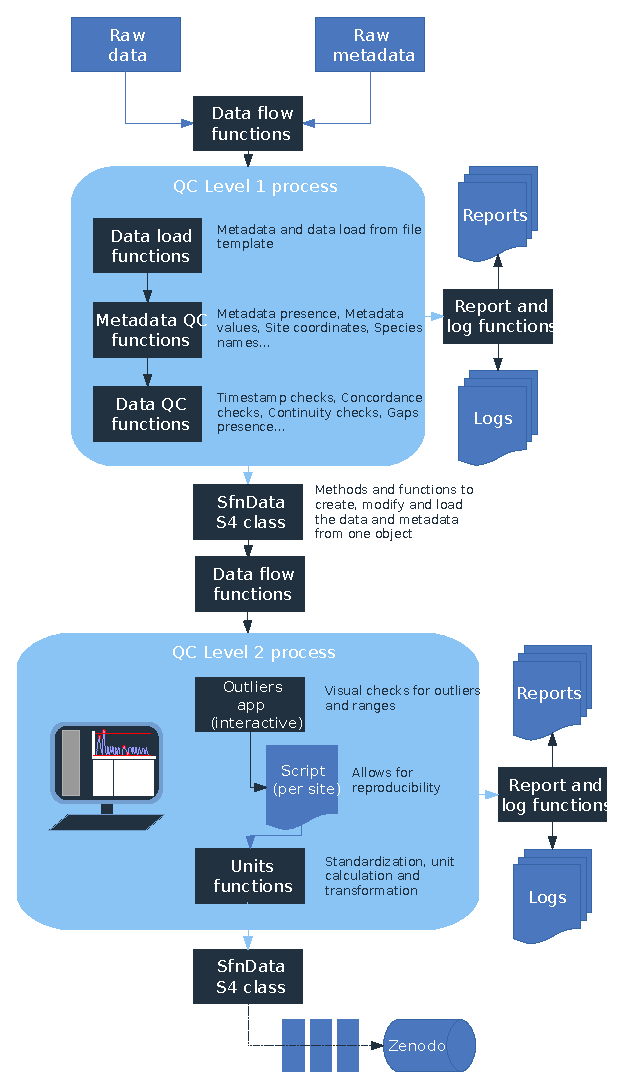
\includegraphics[width=0.7\linewidth]{figure/CH3/Figure1} 

}

\caption[Overview of the SAPFLUXNET data workflow.]{Overview of the SAPFLUXNET data workflow. Data files are received from data contributors, and undergo several quality-control processes (QC1 and QC2). Both, QC1 and QC2 produce an .RData object of the custom-designed sfn-data S4 class storing all data, metadata and data flags for each dataset. The progress and results of the QC processes are monitored through individual reports and log files. The final outcome, is stored in a folder structure with a either single .RData file for each dataset or a set of seven csv files for each dataset.}\label{fig:Ch2plot1}
\end{figure}
\subsection{Data harmonisation and quality control:
QC2}\label{data-harmonisation-and-quality-control-qc2}

Datasets entering QC2 underwent several data cleaning and data
harmonisation processes (Supplement Table S2). We first ran outlier
detection and out of range checks; these checks did not delete or modify
the data, only warned about any suspicious observation (`outlier' and
`range' warnings). The outlier detection algorithm was based on a Hampel
filter, which also estimates a replacement value for a candidate outlier
(Hampel, 1974). For the range checks, we defined minimum and maximum
allowed values for all the time series variables, based on published
values of extreme weather records and maximum transpiration rates
(Cerveny et al., 2007; Manzoni et al., 2013). The outcome of outlier and
range checks were visually inspected on the actual time series being
evaluated using an interactive R Shiny application (Supplement Fig.S3).
Following expert knowledge, visually confirmed outliers were replaced by
the values estimated by the Hampel filter. Similarly, we replaced out of
range values by NA if the variable was out of its physically allowed
range (Supplement Fig.S3). Outlier and out of range `warnings' for each
observation (e.g.~for each variable and timestep) were documented in two
data flags tables, with the same dimensions as the corresponding data
tables (Supplement Fig. S2). Likewise, those observations with confirmed
problematic values, which were removed or replaced, were also flagged;
further information can be found in the `data flags' vignettes in the
`sapfluxnetr' package Granda et al. (Granda et al., 2019)\par

Final data harmonisation processes in QC2 involved unit transformations
and the calculation of derived variables (Supplement Table S2). When
plant sapwood area was provided by data contributors, we interconverted
between sap flow rate per plant and per unit sapwood area. If leaf area
was supplied, we also calculated sap flow per unit leaf area, but note
that this transformation does not take into account the seasonal
variation in leaf area. In QC2 we estimated missing environmental
variables which could be derived from related variables in the dataset
(Appendix, Table A6). We also estimated the apparent solar time and
extraterrestrial global radiation from the provided timestamp and
geographic coordinates using the R package `solaR' (Perpiñán, 2012). All
estimated or interconverted observations were flagged as `CALCULATED' in
the `env\_flags' or `sap\_flags' table (Supplement Fig. S2).\par

\subsection{Data structure}\label{data-structure}

One of the major benefits of the SAPFLUXNET data workflow is the
encapsulation of datasets in self-contained R objects of the S4 class
with a predefined structure. These objects belong to the custom-designed
`sfn\_data' class, which display different slots to store time series of
sap flow and environmental data, their associated data flags, and all
the metadata (Supplement Fig. S2). For further information please see
the `sfn\_data classes' vignette in the `sapfluxnetr' package (Granda et
al., 2019). The code identifying each dataset was created by the
combination of a `country' code, a `site' code and, if applicable, a
`stand' code and a `treatment' code. This means that several `stands'
and/or `treatments' can be present within one `site' (Supplement Table
S3).\par

At the end of the QC process, we generated a folder structure with a
first-level storing datasets as either `sfn\_data' objects or as a set
of comma-separated (csv) text files. Within each of these formats, a
second-level folder groups datasets according to how sap flow is
normalized (per plant, sapwood or leaf area); note that the same
dataset, expressing different sap flow quantities, can be present in
more than one folder (e.g. `plant' and `sapwood'). Finally, the third
level contains the data files for each dataset: either a single
`sfn\_data' object storing all data and metadata, or all the individual
csv files. More details on the data structure can be found in the
`sapfluxnetr-quick-guide' vignette in the `sapfluxnetr' package (Granda
et al., 2019).\par

\section{The SAPFLUXNET database}\label{the-sapfluxnet-database}

\subsection{Data coverage}\label{data-coverage}

The SAPFLUXNET version 0.1.5 database harbours 202 globally distributed
datasets (Fig. 2a, Supplement Fig. S4 and Table S3), from 121
geographical locations, with Europe, Eastern USA and Australia
especially well represented. These datasets were represented in the
bioclimatic space using the terrestrial biomes delimited by Whittaker
(Fig. 2b), but note that, as any bioclimatic classification, it has its
limitations. Datasets have been compiled from all terrestrial biomes,
except for temperate rainforests, although some tropical montane sites
have been included. Woodland/shrubland and temperate forest biomes are
the most represented in the database adding up to 80\% of the datasets
(Fig. 2b). However, large forested areas in the tropics and in boreal
regions are still not well represented (Fig. 2a,b). Looking at the
distribution by vegetation type (Fig. 2c), evergreen needleleaf forest
is the most represented vegetation type (65 datasets), followed by
deciduous broadleaf forest (47 datasets) and evergreen broadleaf forest
(43 datasets).\par

SAPFLUXNET contains sap flow data for 2714 individual plants (1584
angiosperms and 1130 gymnosperms), belonging to 174 species (141
angiosperms and 33 gymnosperms), 95 different genera and 45 different
families (Supplement, Table S4-S5). All species but one, Elaeis
guineensis, a palm, are tree species. Pinus and Quercus are the most
represented genera (Fig. 3b). Amongst the gymnosperms, Pinus sylvestris,
Picea abies and Pinus taeda are the three most represented species with
data provided on 290, 178 and 107 trees, respectively (Fig. 3a). For the
angiosperms, Acer saccharum, Fagus sylvatica and Populus tremuloides are
the most represented species, with 162, 116 and 104 trees, respectively,
although most Acer saccharum data come from a single study with a very
large sample size (Fig. 3a). Some species are present in more than 10
datasets: Pinus sylvestris, Picea abies, Fagus sylvatica, Acer rubrum,
Liriodendron tulipifera and Liquidambar styraciflua (Fig. 3a, Supplement
Table S4).\par

\setlength{\abovecaptionskip}{0pt}
\begin{figure}[H]

{\centering 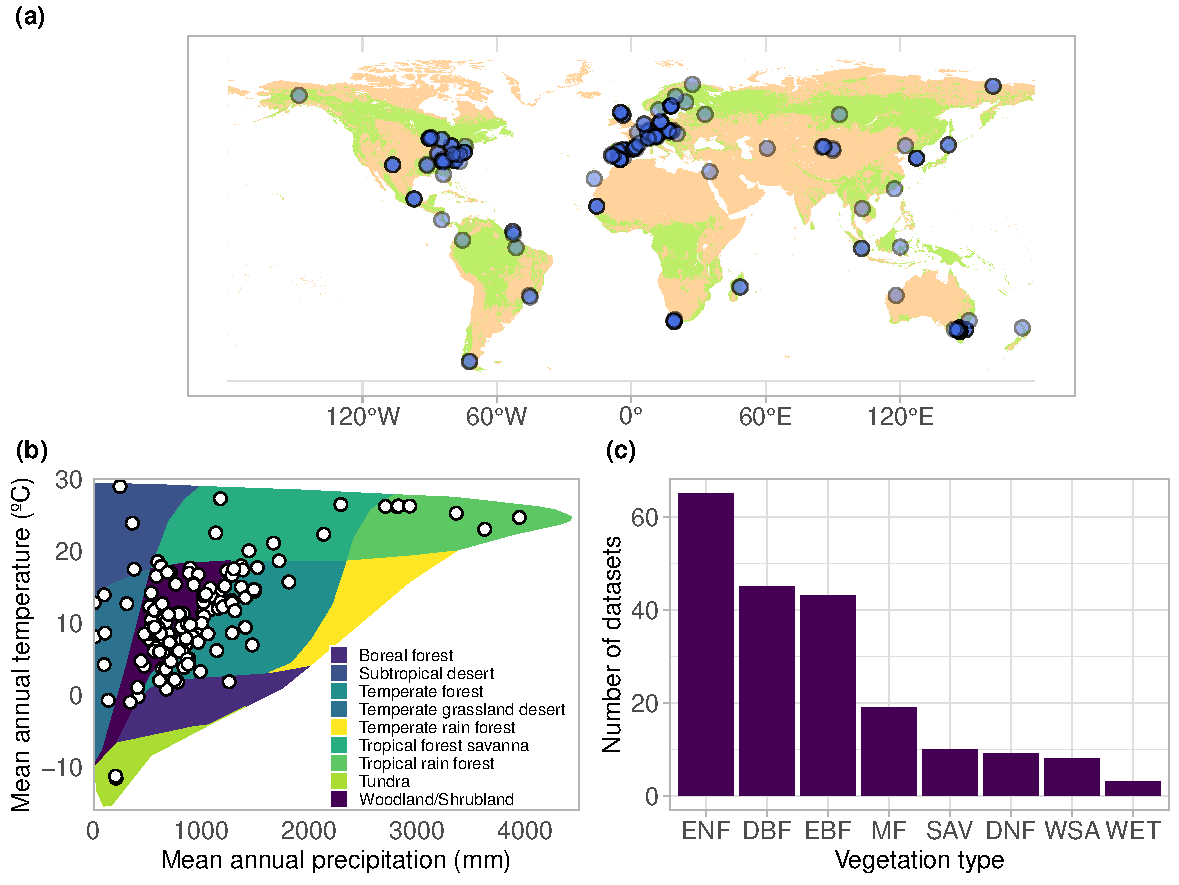
\includegraphics[width=1\linewidth]{figure/CH3/Figure2} 

}

\caption[Geographic, bioclimatic and vegetation type distribution of SAPFLUXNET datasets.]{(a) Geographic, (b) bioclimatic and (c) vegetation type distribution of SAPFLUXNET datasets. In (a) woodland area from Crowther et al. (2015) is shown in green. In (b) we represent the different datasets according to their mean annual temperature and precipitation in a Whittaker diagram showing the classification of the main terrestrial biomes. In (c) vegetation types are defined according to the International Geosphere-Biosphere Programme (IGBP) classification (ENF: Evergreen Needleleaf Forest; DBF: Deciduous Broadleaf Forest; EBF: Evergreen Broadleaf Forest; MF: Mixed Forest; DNF: Deciduous Needleleaf forest; SAV: Savannas; WSA: Woody Savannas; WET: Permanent Wetlands).}\label{fig:Ch2plot2}
\end{figure}
\setlength{\abovecaptionskip}{0pt}
\begin{figure}[H]

{\centering 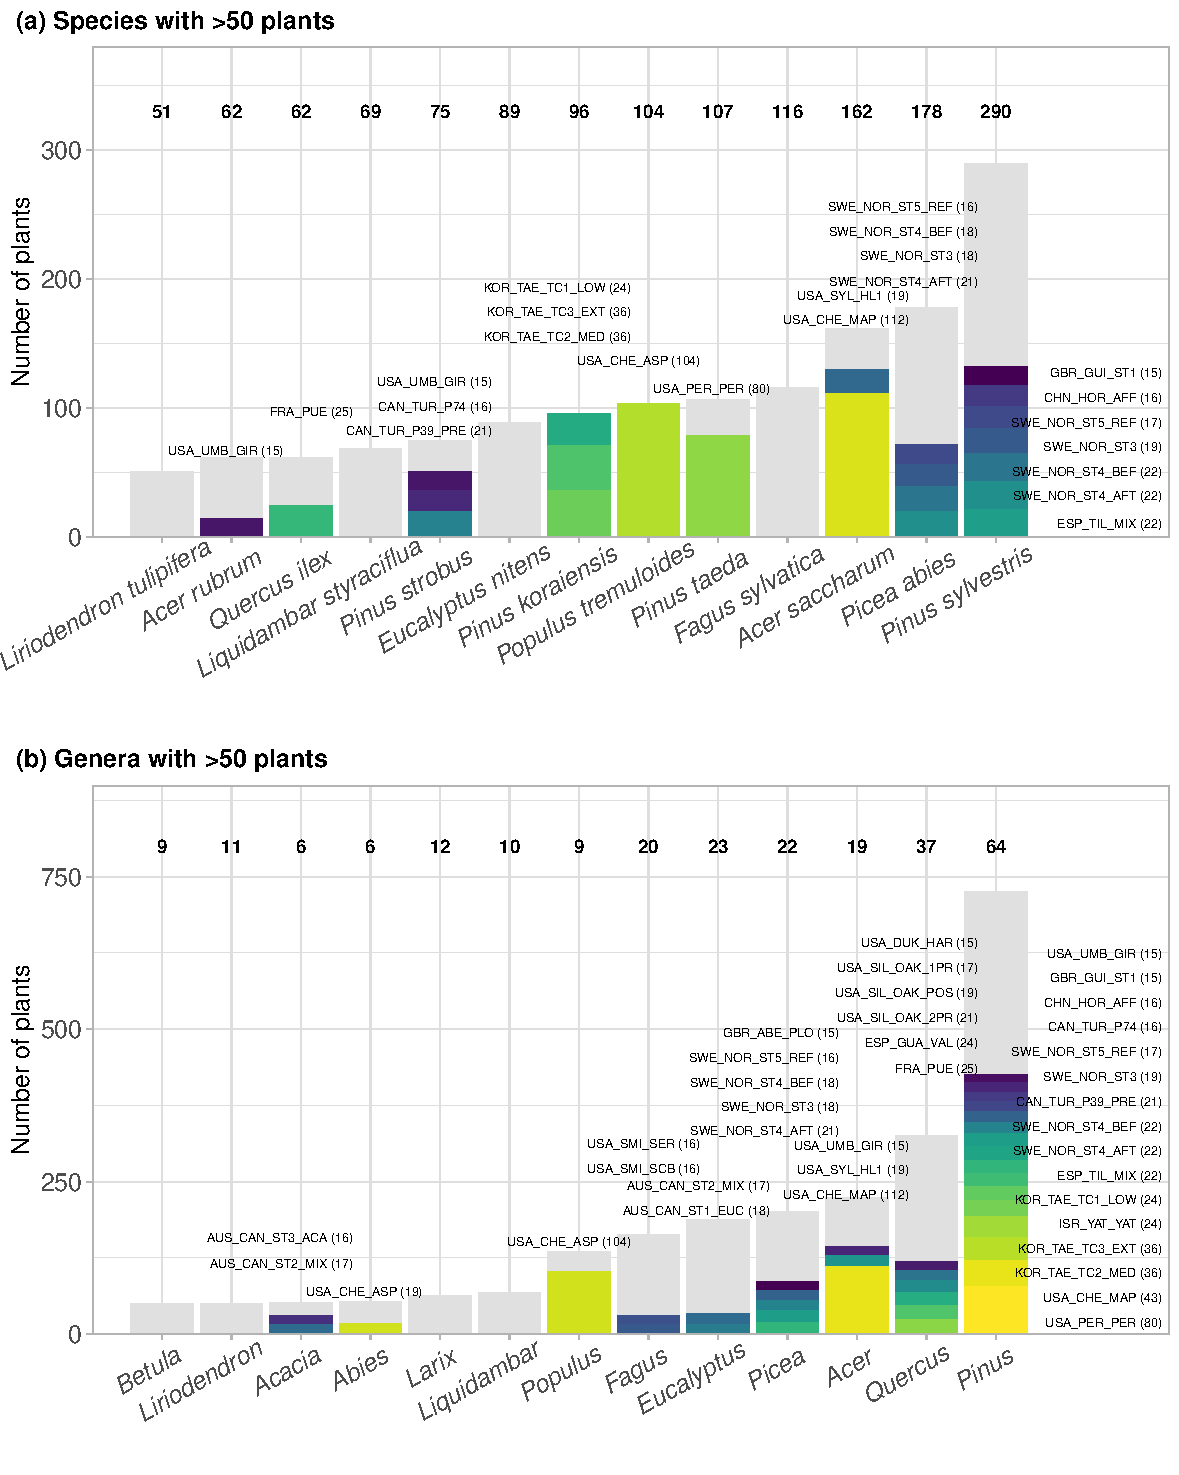
\includegraphics[width=1\linewidth]{figure/CH3/Figure3} 

}

\caption[Taxonomic distribution of genera and species in SAPFLUXNET.]{Taxonomic distribution of genera and species in SAPFLUXNET, showing (a) species and (b) genera with > 50 plants in the database. Total bar height depicts number of plants per species (a) or genera (b). Numbers on top of each bar show the number of datasets where each species (a) or genus (b) is present. Colours other than grey highlight datasets with 15 or more plants of a given species (a) or genus (b). Bar height for a given colour is proportional to the number of plants in the corresponding dataset, which is also shown in parentheses next to the dataset code.}\label{fig:Ch2plot3}
\end{figure}
\subsection{Methodological aspects}\label{methodological-aspects}

For more than 90\% of the plants, sap flow at the whole-plant level is
available (either directly provided by contributors or calculated in the
QC process); this is important for upscaling SAPFLUXNET data to the
stand level (cf.~section 4.2). Because the leaf area of the measured
plants is often not available as metadata, sap flow per unit leaf area
was estimated for only 18.6\% of the individuals (Fig. 4). The heat
dissipation method is the most frequent method in the database (HD,
66.4\% of the plants), followed by the trunk sector heat balance (TSHB,
16.4\%) and the compensation heat pulse method (CHP, 8.4\%) (Fig. 4).
This distribution is broadly similar to the use of each method
documented in the literature, although the TSHB method is
overrepresented here, compared to the current use of this method by the
sap flow community (Flo et al., 2019; Poyatos et al., 2016). Some
methods, especially those belonging to the heat pulse family and the
cyclic (or transient) heat dissipation (CHD) method are mostly used in
angiosperms, while the TSHB and the heat field deformation (HFD) methods
are more frequently used in gymnosperms (Fig. 4).\par

\setlength{\abovecaptionskip}{0pt}
\begin{figure}[hbt!]

{\centering 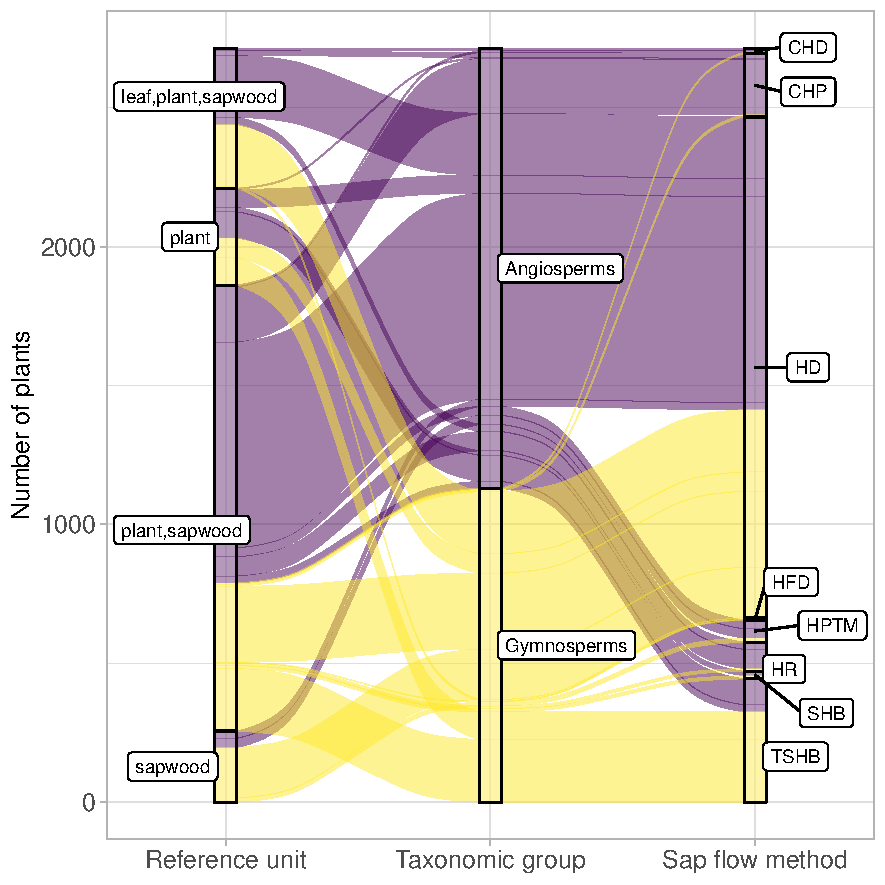
\includegraphics[width=1\linewidth]{figure/CH3/Figure4} 

}

\caption[Distribution of plants according to major taxonomic group and sap flow method.]{Distribution of plants in SAPFLUXNET according to major taxonomic group (angiosperms, gymnosperms), sap flow method (CHD:cycling heat dissipation; CHP: compensation heat pulse; HD: heat dissipation; HFD: heat field deformation: HPTM: heat pulse T-max (HPTM): HRM: heat ratio (HR); SHB: stem heat balance; TSHB: trunk sector heat balance) and reference unit for the expression of sap flow (plant, sapwood area, leaf area). Combinations of reference units imply that data are present in multiple units.}\label{fig:Ch2plot4}
\end{figure}
Calibration of sap flow sensors and scaling from point measurements to
the whole-plant can be critical steps towards accurate estimates of
absolute sap flow rates. In SAPFLUXNET, most of the sap flow time series
have not undergone a species-specific calibration, with the CHD method
showing the highest percentage of calibrated time series (Table 1). This
lack of calibrations may be relevant for the more empirical heat
dissipation methods (HD and CHD), which have been shown to consistently
underestimate sap flow rates (Flo et al., 2019; Peters et al., 2018;
Steppe et al., 2010). Radial integration of single-point sap flow
measurements is more frequent than azimuthal integration (Table 2),
except for the CHD method. A large number of plants using the HD method,
and all plants measured using the HPTM method, do not employ any radial
integration procedure. In contrast, the CHP, HR, SHB, and TSHB methods
are those which more frequently addressed radial variation in one way or
another (Table 2). Azimuthal integration procedures are also more
frequent when the TSHB method is used (Table 2).\par
\begin{table}[!h]

\caption[Number of sap flow times series in SAPFLUXNET depending on whether they were calibrated for the different sap flow methods.]{\label{tab:Ch3T1}Number of sap flow times series in SAPFLUXNET depending on whether they were calibrated (species-specific), non-calibrated or this information was not provided, for the different sap flow methods: cyclic (or transient) heat dissipation (CHD), compensation heat pulse (CHP), heat dissipation (HD), heat field deformation (HFD), heat pulse T-max (HPTM), heat ratio (HR), stem heat balance (SHB) and trunk sector heat balance (TSHB). The percentage of calibrated time series was expressed with respect to the total number of sap flow time series for each method.}
\centering
\fontsize{10}{12}\selectfont
\begin{tabular}[t]{ccccc}
\toprule
Method & Calibrated & Non-calibrated & Not provided & \% calibrated\\
\midrule
CHD & 6 & 13 & 0 & 31.6\\
CHP & 29 & 42 & 157 & 12.7\\
HD & 214 & 1491 & 98 & 11.9\\
HR & 3 & 55 & 47 & 2.9\\
TSHB & 7 & 433 & 4 & 1.6\\
HFD & 0 & 8 & 0 & 0.0\\
HPTM & 0 & 80 & 0 & 0.0\\
SHB & 0 & 27 & 0 & 0.0\\
\bottomrule
\end{tabular}
\end{table}
\begin{table}

\caption[Number of plants in the SAPFLUXNET database using different radial and azimuthal integration.]{\label{tab:Ch3T2}Number of plants in the SAPFLUXNET database using different radial and azimuthal integration approaches for the different sap flow methods: cyclic (or transient) heat dissipation (CHD), compensation heat pulse (CHP), heat dissipation (HD), heat field deformation (HFD), heat pulse T-max (HPTM), heat ratio (HR), stem heat balance (SHB) and trunk sector heat balance (TSHB).}
\centering
\resizebox{\linewidth}{!}{
\fontsize{10}{12}\selectfont
\begin{tabular}[t]{ccc>{\centering\arraybackslash}p{3.5cm}>{\centering\arraybackslash}p{2.5cm}c}
\toprule
\multicolumn{6}{l}{\textbf{Azimuthal integration}} \\
\cmidrule(l{3pt}r{3pt}){1-6}
Method & Measured & Sensor-integrated & Corrected, measured azimuthal variation & No azimuthal correction & Not provided\\
\midrule
CHD & 15 & 0 & 0 & 0 & 4\\
CHP & 61 & 0 & 0 & 167 & 0\\
HD & 216 & 0 & 520 & 1021 & 46\\
HFD & 0 & 0 & 0 & 8 & 0\\
HPTM & 0 & 0 & 0 & 80 & \vphantom{1} 0\\
HR & 7 & 0 & 2 & 88 & 8\\
SHB & 0 & 0 & 0 & 27 & 0\\
TSHB & 0 & 25 & 191 & 219 & 9\\
\addlinespace[0.5em]
\hline
\multicolumn{6}{l}{\textbf{Radial integration}}\\
\hline
\hspace{1em}Method & Measured & Sensor-integrated & Corrected, measured radial variation & No radial correction & Not provided\\
\hline
\hspace{1em}CHD & 0 & 0 & 6 & 13 & 0\\
\hspace{1em}CHP & 222 & 0 & 6 & 0 & 0\\
\hspace{1em}HD & 77 & 3 & 645 & 703 & 142\\
\hspace{1em}HFD & 2 & 0 & 0 & 6 & 0\\
\hspace{1em}HPTM & 0 & 0 & 0 & 80 & 0\\
\hspace{1em}HR & 57 & 1 & 42 & 3 & 2\\
\hspace{1em}SHB & 0 & 27 & 0 & 0 & 0\\
\hspace{1em}TSHB & 0 & 338 & 8 & 89 & 9\\
\bottomrule
\end{tabular}}
\end{table}
\subsection{Plant characteristics}\label{plant-characteristics}

Plant-level metadata is almost complete (99.5\% of the individuals) for
diameter at breast height (DBH), while sapwood area and sapwood depth,
important variables for sap flow upscaling, are not available, or could
not be estimated, for 23\% and 47\% of the plants, respectively. Plant
height and plant age are missing for 42\% and 62\% of the individuals,
respectively. Sap flow data in SAPFLUXNET are representative of a broad
range of plant sizes (Fig. 5a). The distribution of DBH showed a median
of 25.0 cm and 20.4 cm for gymnosperms and angiosperms, respectively,
with a long tail towards the largest plants, two Mortoniodendron
anisophyllum trees from a tropical forest in Costa Rica that measured
\textgreater{} 200 cm (Fig. 5a). The largest gymnosperm tree in
SAPFLUXNET (176 cm in DBH) is a kauri tree (Agathis australis) from New
Zealand. The distribution of plant heights is less skewed, with similar
medians for angiosperms (17.6 m) and gymnosperms (17.5 m). The tallest
plants are located in a tropical forest in Indonesia, where a Pouteria
firma tree reached 44.7 m. Remarkably, of the 16 plants taller than 40
m, over 60\% are Eucalyptus species. The tallest gymnosperm (36.2 m) is
a Pinus strobus from NE USA.\par

\setlength{\abovecaptionskip}{0pt}
\begin{figure}[hbt!]

{\centering 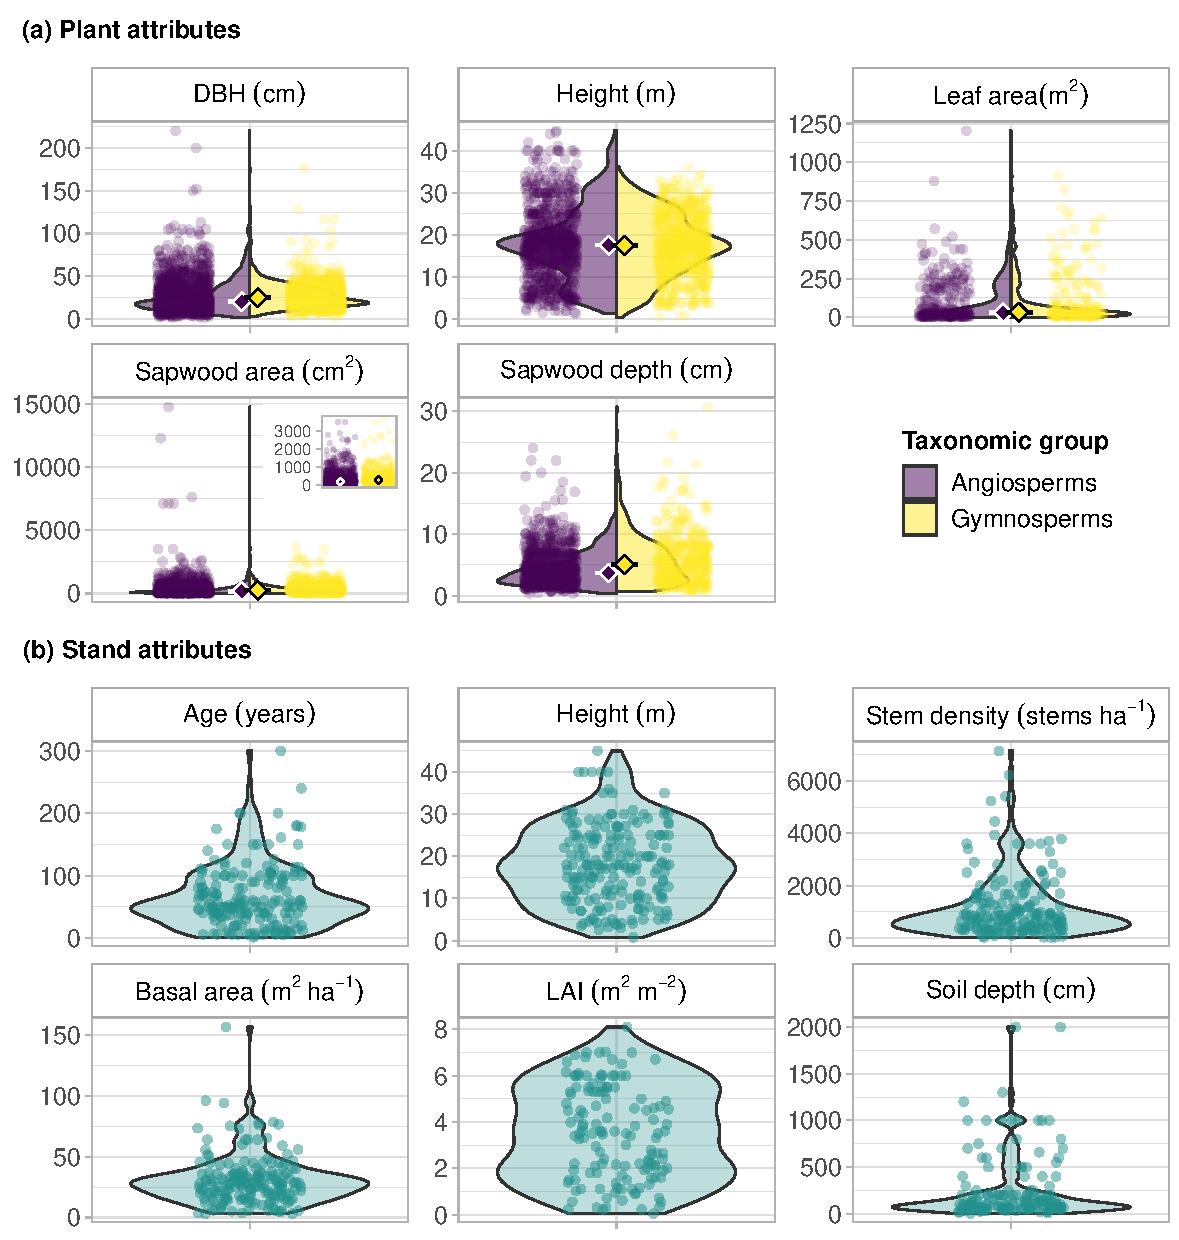
\includegraphics[width=1\linewidth]{figure/CH3/Figure5} 

}

\caption[Characteristics of trees and stands in the SAPFLUXNET database.]{Characteristics of trees and stands in the SAPFLUXNET database. Panel (a) shows plant data and kernel density plots of the main plant attributes, coloured by taxonomic group (angiosperms and gymnosperms): diameter at breast height (DBH), plant height, sapwood area, sapwood depth and leaf area. The inset in the sapwood area panel zooms in values lower than 5000 cm². Panel (b) shows stand data and kernel density plots of the main stand attributes: stand age, stand height, stem density, stand basal area,leaf area index (LAI) and soil depth.}\label{fig:Ch2plot5}
\end{figure}
Plant size metadata in SAPFLUXNET is complemented with plant-level data
of sapwood and leaf area, that provide information on the functional
areas for water transport and loss (Fig. 5a). Distributions of sapwood
and leaf area show highly skewed distributions, with long tails towards
the largest values and slightly higher median values for gymnosperms
(262 cm2 and 33.0 m2 for sapwood and leaf areas, respectively), compared
to angiosperms (168 cm2 and 29.9 m2). Accordingly, median sapwood depth
is also higher for gymnosperms (5.1 cm) compared to angiosperms (3.7
cm). The largest trees (Mortoniodendron, Pouteria, Agathis) with deep
sapwood (17--24 cm) are also those with largest sapwood areas. Many
large angiosperm trees from tropical (CRI\_TAM\_TOW, IDN\_PON\_STE,
GUF\_GUY\_ST2; see Table S3 for dataset codes) and temperate forests
(Fagus grandifolia, USA\_SMIC\_SCB) also show large sapwood areas
(\textgreater{} 5000 cm2), but the plant with the deepest sapwood is a
gymnosperm, an Abies pinsapo in Spain with 30.7 cm of sapwood depth.\par

\subsection{Stand characteristics}\label{stand-characteristics}

Stand-level metadata include several variables associated with
management, vegetation structure and soil properties. Half of the
datasets originate from naturally regenerated, unmanaged stands, and
13.9\% come from naturally regenerated but managed stands. Plantations
add up to 32.2\% and orchards only represent 4\% of the datasets.
Reporting of structural variables is mixed, with stand height, age,
density and basal area showing relatively low missingness (6.4\%,
11.4\%, 12.9\% and 13.4\%, respectively); in contrast, soil depth and
LAI are missing from 26.7\% and 33.7\% of the datasets.\par

SAPFLUXNET datasets originate from stands with diverse structural
characteristics. Median stand age is 54 years and there are several
datasets coming from \textgreater{}100 year-old forests (Fig. 5b). Stand
height shows a similar range and distribution of values compared to
individual plant height (Fig. 5a,b). The denser stands correspond to
coppiced evergreen oak stands from Mediterranean forests (FRA\_PUE,
ESP\_TIL\_OAK), species-rich tropical forests (MDG\_SEM\_TAL) or
relatively young temperate forests (e.g.~FRA\_HES\_HE1\_NON,
USA\_CHE\_MAP). The sparsest stands (\textless{} 200 stems ha-1)
correspond to tree-grass savanna systems (Spain, Portugal, Australia,
Senegal), dry woodlands (China), or oil palm plantations in Indonesia
(IDN\_JAM\_OIL). Stands with the largest basal areas (\textgreater{} 70
m2 ha-1) are mostly dominated by broadleaf species, except for a Picea
abies plantation in Sweden (SWE\_SKO\_MIN).\par

The distribution of leaf area index (LAI) shows a median of 3.5 m2 m-2,
with the largest values observed in temperate (CZE\_BIK, USA\_DUK\_HAR,
HUN\_SIK) and tropical (GUF\_GUY\_GUY, COL\_MAC\_SAF\_RAD) forests. The
stands with the lowest LAI correspond to the sparse woodlands from
Mediterranean and semi-arid locations and also those from forests near
altitudinal or latitudinal tree-lines (FIN\_PET, AUT\_TSC). SAPFLUXNET
datasets show a median soil depth of 100 cm, with only a dozen datasets
originated from sites with soils deeper than 10 m (Fig. 5b).\par

The number of plants per dataset is highly variable, with most of the
datasets (86\%) containing data for at least 4 trees and 46\% of the
datasets having data for at least 10 trees (Fig. 6a, see also Fig. 9).
\par

\setlength{\abovecaptionskip}{0pt}
\begin{figure}[hbt!]

{\centering 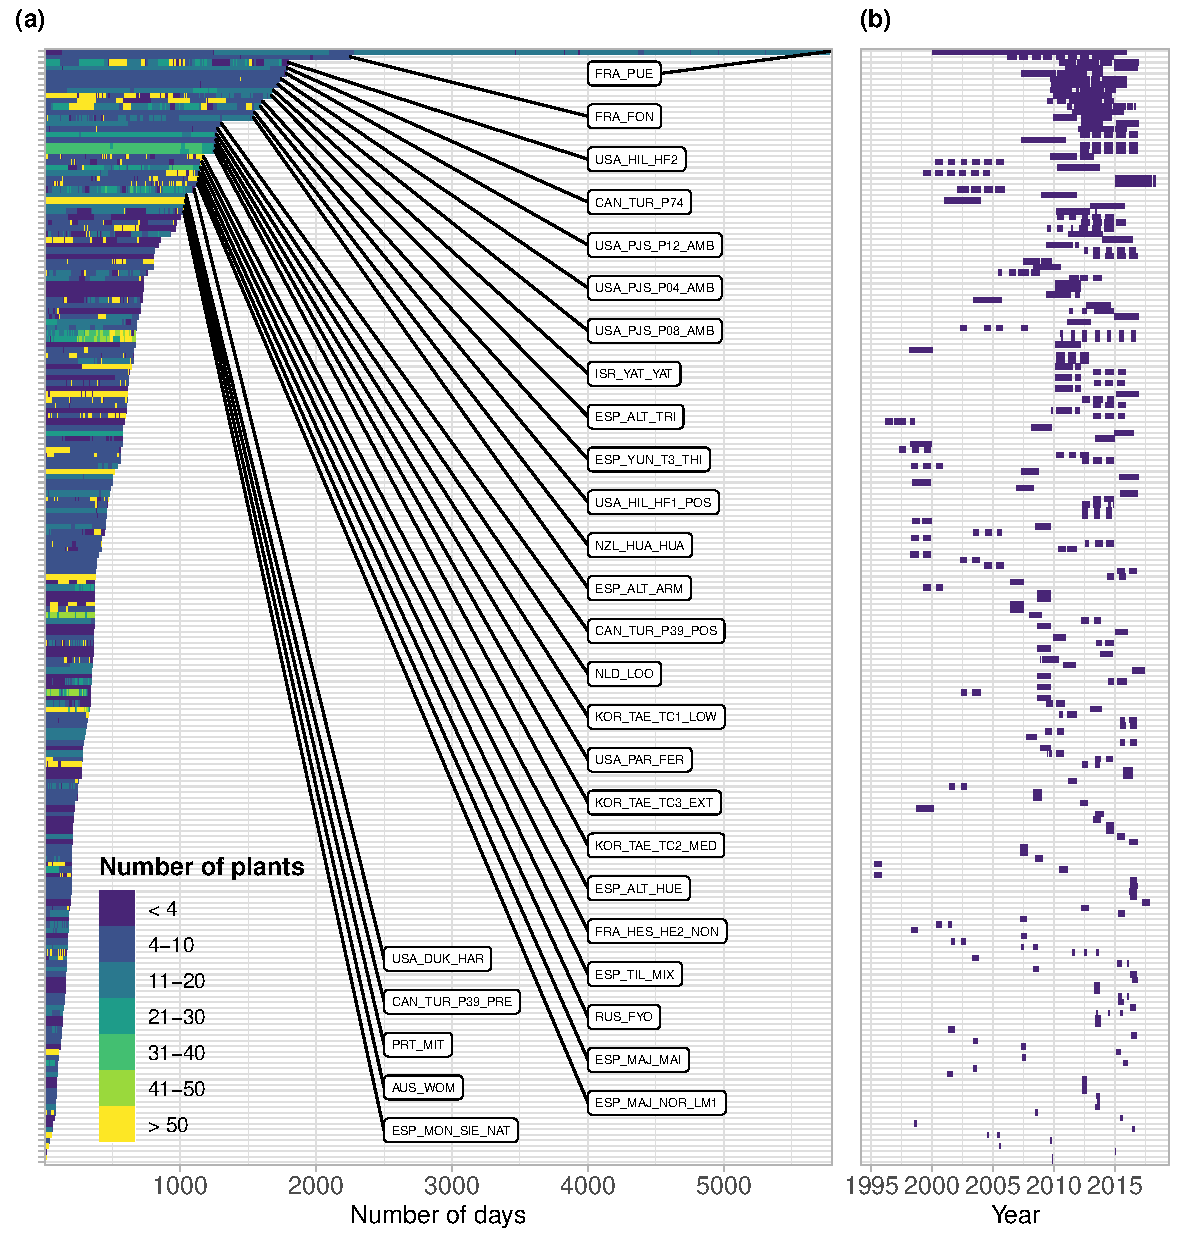
\includegraphics[width=1\linewidth]{figure/CH3/Figure6} 

}

\caption[Duration and number of plants mesured in each dataset.]{(a) Measurement duration of SAPFLUXNET datasets expressed in number of days with sap flow data and coloured by the number of plants measured on each day . The 30 longest datasets are labelled. For each dataset in panel (a), panel (b) shows its corresponding measurement period.}\label{fig:Ch2plot6}
\end{figure}
\subsection{Temporal characteristics}\label{temporal-characteristics}

The oldest datasets in SAPFLUXNET go back to 1995 (GBR\_DEV\_CON,
GBR\_DEV\_DRO) while the most recent data reach up to 2018 (datasets
from the ESP\_MAJ cluster of sites). Several multi-year datasets are
present in SAPFLUXNET (Fig. 6), with 50\% of the datasets spanning a
period of at least 3 years, and some datasets being extraordinarily long
(16 years in FRA\_PUE). Frequently, the datasets only cover the `growing
season' periods, or even shorter periods for some sites which were
eventually included because they improved the ecological and geographic
coverage of the database (e.g.~ARG\_MAZ, ARG\_TRE as representative of
deciduous Nothofagus forest in South Patagonia). In contrast, a few
datasets show continuous records over multiple years (Fig. 6b). Amongst
the longest datasets, most of them come from European or North American
sites (Fig. 6), except some datasets from Israel (ISR\_YAT\_YAT, 7
years), Russia (RUS\_FYO, 7 years), South Korea (KOR\_TAE cluster of
sites, 6 years) or New Zealand (NZL\_HUA\_HUA, 5 years).\par 

SAPFLUXNET provides an unprecedented database to study the detailed
temporal dynamics of plant transpiration across species and sites
globally. Sub-daily records of sap flow (e.g.~at least at hourly
timesteps) are available for extended periods (Fig. 6b), allowing to
address both seasonal and diel patterns in water use regulation by trees
and how these temporal patterns change across species or years across
terrestrial biomes, reflecting different phenologies and water-use
strategies. For instance, in Mediterranean forests, evergreen species
such as Quercus ilex, Arbutus unedo and Pinus halepensis show moderate
sap flow the whole year round, while the deciduous Quercus pubescens
shows higher sap flow density during a shorter period and its water use
is heavily reduced during a dry year (2012) (Fig. 7a). Temperate forests
without water availability limitations show relatively high flows during
the growing season and similar diel sap flow patterns among species
(Fig. 7b). In contrast, tropical forests show moderate to high sap flow
rates during the entire year, with different dynamics in the intradaily
water use regulation across species. For example, Inga sp. in a highly
diverse wet tropical forest in Costa Rica, reduced sap flow during
mid-day hours compared to co-existing species (Fig. 7c).\par

\setlength{\abovecaptionskip}{0pt}
\begin{figure}[hbt!]

{\centering 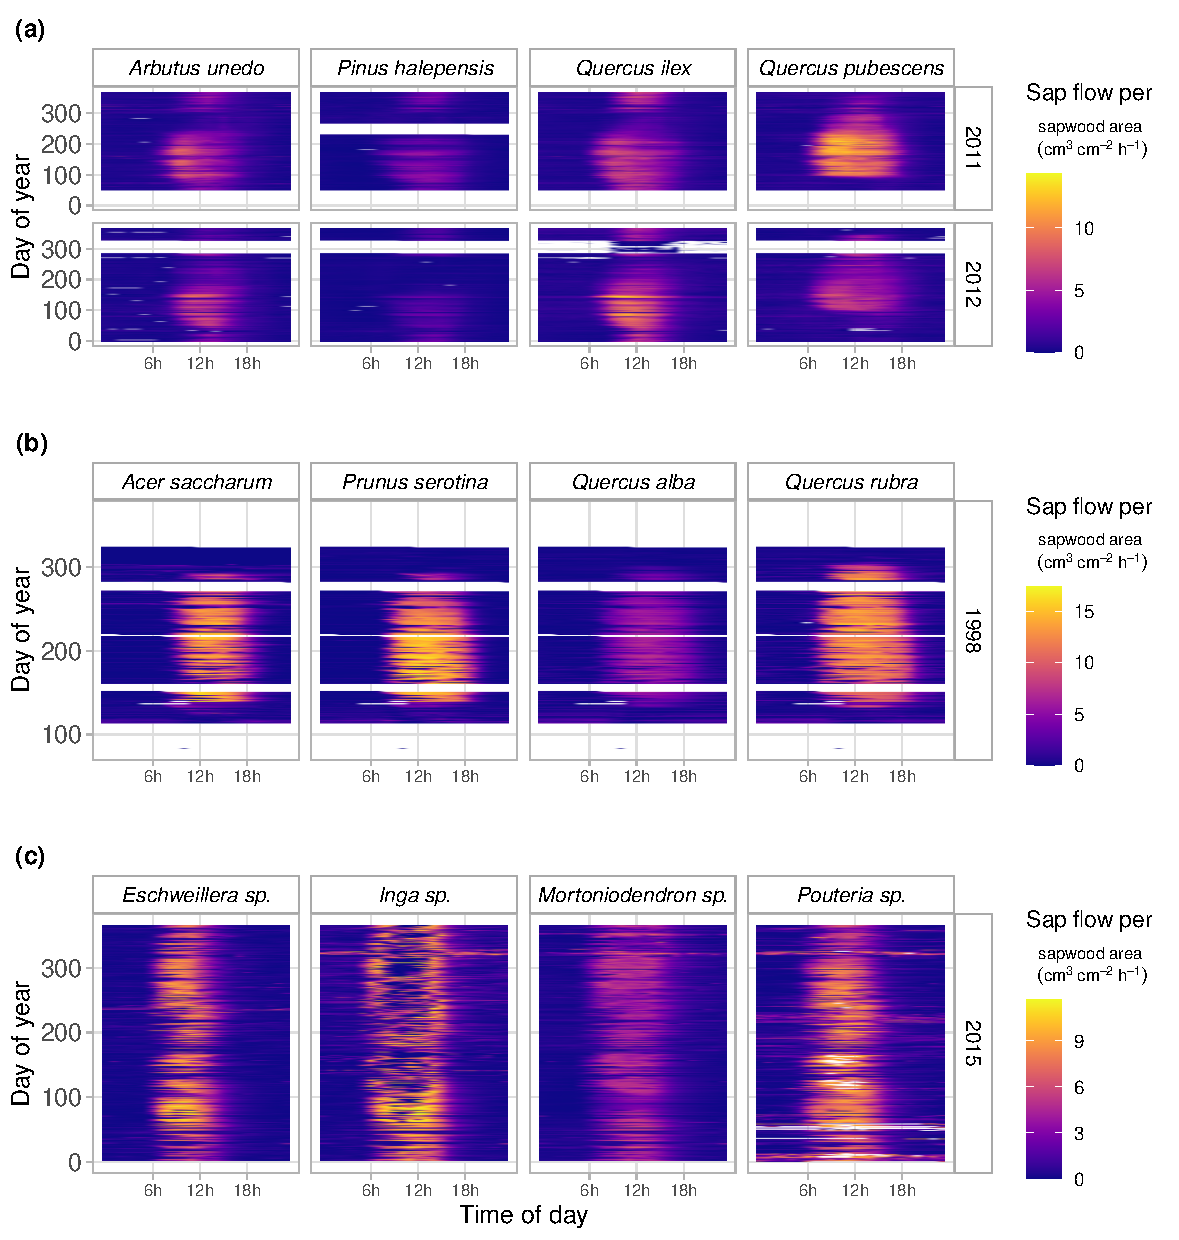
\includegraphics[width=1\linewidth]{figure/CH3/Figure7} 

}

\caption[Fingerprint plots showing hourly sap flow per unit sapwood area.]{Fingerprint plots showing hourly sap flow per unit sapwood area (colour scale) as a function of hour of day (x-axis) and day of year (y-axis) for a selection of SAPFLUXNET sites with at least four co-occurring species. Panel (a) shows data from a Woodland/Shrubland forest in NE Spain (ESP\_CAN), for an average (2011) and a dry (2012) year. Panel (b) shows data for a mesic Temperate forest (USA\_WVF) and panel (c) shows data for a Tropical forest (CRI\_TAM\_TOW). For this latter site, only 4 of the 17 measured species are shown and some of them were only identified at the genus level.}\label{fig:Ch2plot7}
\end{figure}
\subsection{Availability of environmental
data}\label{availability-of-environmental-data}

All SAPFLUXNET datasets contain ancillary time series of the main
hydrometeorological drivers of transpiration, accompanied by information
on where these variables had been measured (Fig. 8a). Air temperature is
available for all datasets. Although vapour pressure deficit (VPD) was
originally absent in 38\% of the datasets (Fig. 8a,b), we could estimate
it for those sites providing air temperature and relative humidity data
(QC Level 2, see section 2.3), and finally only 2 out of the 202
datasets have missing VPD information. For radiation variables,
shortwave radiation was most often provided, compared to
photosynthetically active and net radiation; only 8 out of 202 datasets
do not have any accompanying radiation data. Most of these environmental
variables were measured on-site, with precipitation being the variable
most frequently retrieved from nearby meteorological stations (48\% of
the datasets) (Fig. 8a). Soil water content measured at shallow depth,
typically between 0 and 30 cm below the soil surface, is provided for
56\% of the datasets, while soil moisture from deep soil layers is
available for only 27\% of the datasets.\par

\setlength{\abovecaptionskip}{0pt}
\begin{figure}[hbt!]

{\centering 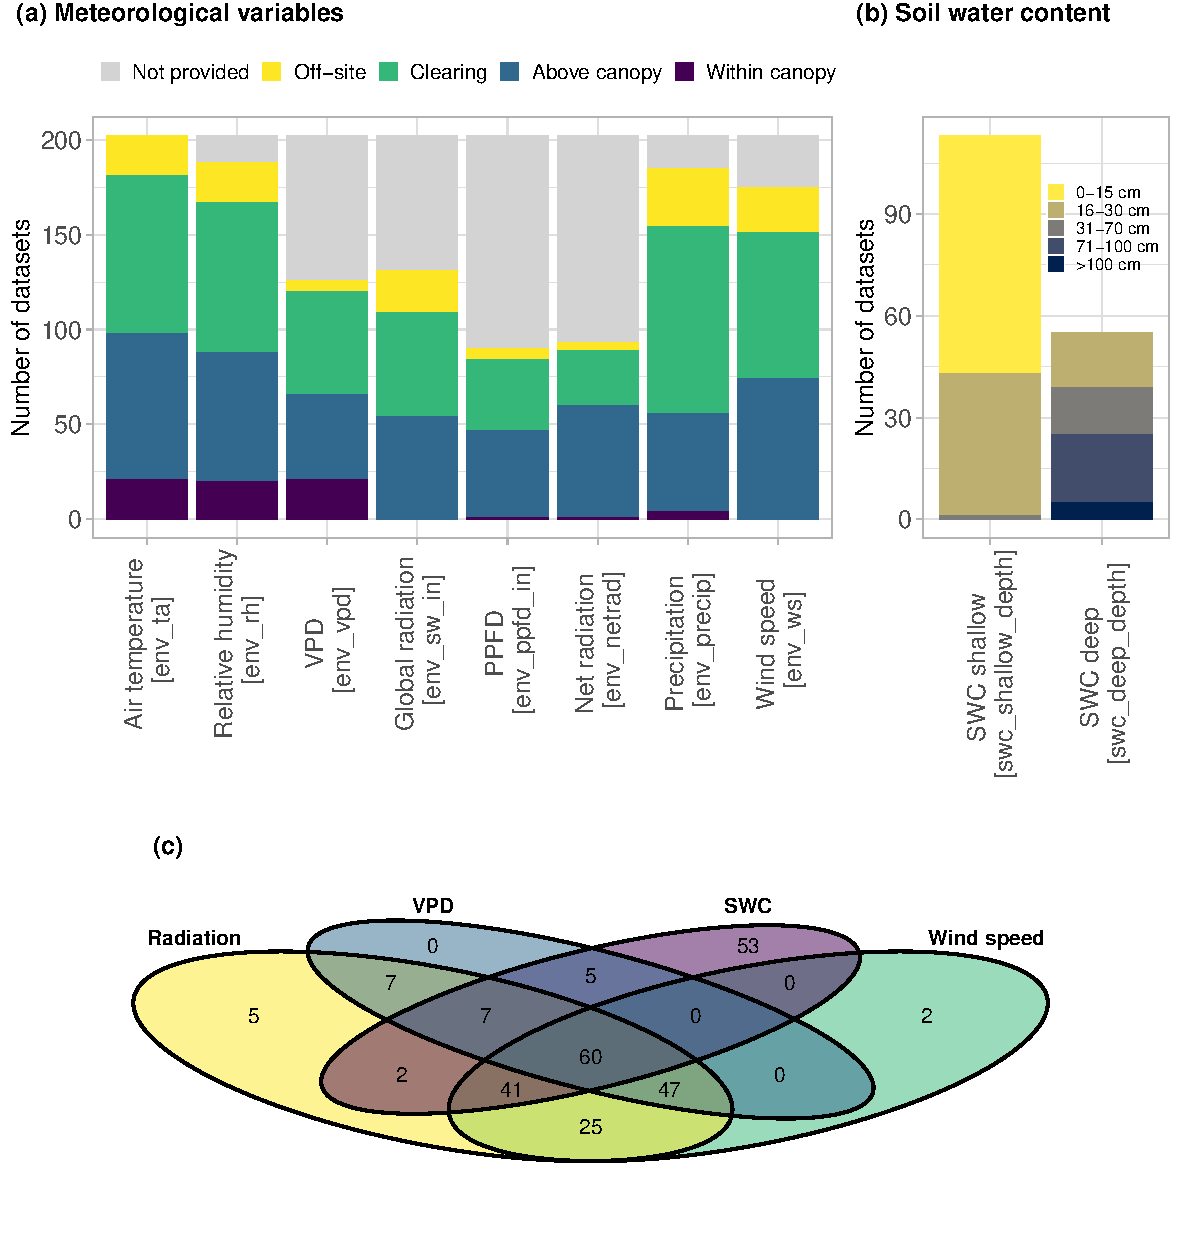
\includegraphics[width=1\linewidth]{figure/CH3/Figure8} 

}

\caption[Summary of the availability of different environmental variables in SAPFLUXNET datasets.]{Summary of the availability of different environmental variables in SAPFLUXNET datasets. (a) Distribution of meteorological variables according to sensor location (in brackets, names of the variables in the database), (b) Distribution of soil moisture variables according to the measurement depth (in brackets, names of the variables in the database). (c) Venn diagram showing the number of datasets where each combination of different environmental variables are present, grouping shortwave, PPFD and net radiation under ‘Radiation’ variables.}\label{fig:Ch2plot8}
\end{figure}
\section{Potential applications}\label{potential-applications}

\subsection{Applications in plant ecophysiology and functional
ecology}\label{applications-in-plant-ecophysiology-and-functional-ecology}

There are multiple potential applications of the SAPFLUXNET database to
assess whole-plant water use rates and their environmental sensitivity,
both across species (e.g.~Oren et al., 1999b) and at the intraspecific
level (Poyatos et al., 2007). SAPFLUXNET will allow disentangling the
roles of evaporative demand and soil water content in controlling
transpiration at the plant level, complementing recent studies looking
at how water supply and demand affect evapotranspiration at the
ecosystem level (Anderegg et al., 2018; Novick et al., 2016). The
availability of global sap flow data at sub-daily time resolution and
spanning entire growing seasons will allow focusing on how maximum water
use and its environmental sensitivity varies with plant-level attributes
such as stem diameter (Dierick and Hölscher, 2009; Meinzer et al.,
2005), tree height (Novick et al., 2009; Schäfer et al., 2000),
hydraulic (Manzoni et al., 2013; Poyatos et al., 2007) and other plant
traits (Grossiord et al., 2019; Kallarackal et al., 2013). SAPFLUXNET
thus provides an unprecedented tool to understand how structural and
physiological traits scale-up to whole-plant regulation of water fluxes
(McCulloh et al., 2019), and how this integration determines drought
responses (Choat et al., 2018) and post-drought recovery patterns (Yin
and Bauerle, 2017). Analyses of the temporal dynamics of plant water use
in response to specific drought events, as recently assessed for gross
primary productivity (e.g.~Schwalm et al., 2017), can also help to
quantify drought legacy effects, including the reversibility of
drought-induced losses of hydraulic conductivity at the plant level.\par

SAPFLUXNET will allow new insights into within-day patterns and controls
in whole-plant water use, which can disclose the fine details of its
physiological regulation. Circadian rhythms can modulate stomatal
responses to the environment, potentially affecting sap flow dynamics
(e.g.~de Dios et al., 2015). Hysteresis in diel sap flow relationships
with evaporative demand and time-lags between evaporative demand and sap
flow, are two linked phenomena likely arising from plant capacitance and
other mechanisms (O'Brien et al., 2004; Schulze et al., 1985), that also
influence diel evapotranspiration dynamics (Matheny et al., 2014; Zhang
et al., 2014). A major driver of time-lags is the use of stored water to
meet the transpiration demand (Phillips et al., 2009), which can now be
analysed across species, plant sizes or drought conditions using time
series analyses, simplified electric analogies (Phillips et al., 1997,
2004; Ward et al., 2013) or detailed water transport models (Bohrer et
al., 2005; Mirfenderesgi et al., 2016). Night-time water use can be
substantial for some species (Forster, 2014; Resco de Dios et al.,
2019). However, available syntheses rely on study-specific
quantification of what constitutes nocturnal sap flow and do not address
possible methodological influences (Zeppel et al., 2014). SAPFLUXNET
will allow applying a consistent estimation of nocturnal sap flow and
control for datasets that are less suitable for the quantification of
night-time fluxes, as information on zero-flow determination is included
in the metadata (`pl\_sens\_cor\_zero', Appendix Table A5).\par

Sap flow data have been widely employed to assess changes in tree water
use after biotic (e.g.~Hultine et al., 2010) or abiotic (Oren et al.,
1999a) disturbances. Likewise, sap flow data have been used to report
changes in species and stand water use following experimental treatments
involving resource availability modifications (e.g.~Ewers et al., 1999)
or density changes (i.e.~thinning, Simonin et al., 2007). The SAPFLUXNET
database includes datasets with experimental manipulations, applied
either at the stand or at the individual level (Table 3). The main
treatments present are related to thinning, water availability changes
(irrigation, throughfall exclusion) and wildfire impact (Table 3),
potentially facilitating new data syntheses and meta-analyses using
these datasets (e.g.~Grossiord et al., 2017).\par
\begin{table}[!h]

\caption[Number of datasets, plants and species by stand-level treatment in the SAPFLUXNET database.]{\label{tab:Ch3T3}Number of datasets, plants and species by stand-level treatment in the SAPFLUXNET database.}
\centering
\fontsize{10}{12}\selectfont
\begin{tabular}[t]{cccc}
\toprule
Treatment & N sites & N plants & N species\\
\midrule
None/control & 155 & 2198 & 170\\
Thinning & 18 & 332 & 18\\
Irrigation & 9 & 36 & 4\\
Post-fire & 6 & 18 & 4\\
CO2 fertilisation & 3 & 28 & 2\\
Drought & 3 & 9 & 2\\
Soil fertilisation & 2 & 16 & 2\\
Post-mortality & 1 & 22 & 5\\
Soil fertilisation and pruning & 1 & 12 & 1\\
Soil fertilisation and thinning & 1 & 12 & 1\\
Pruning and thinning & 1 & 11 & 1\\
Soil fertilisation, pruning and thinning & 1 & 11 & 1\\
Pruning & 1 & 9 & 1\\
\bottomrule
\end{tabular}
\end{table}
The combination of SAPFLUXNET with other ecophysiological databases can
inform on the relative sensitivity of different physiological processes
in response to drought, for example those related to growth and carbon
assimilation (Steppe et al., 2015) . Within-day fluctuations of stem
diameter can be jointly analysed with co-located sap flow measurements
to study the dynamics of stored water use under drought and its
contribution to transpiration (e.g.~Brinkmann et al., 2016), and to
infer parameters on tree hydraulic functioning using mechanistic models
of tree hydrodynamics (Salomón et al., 2017; Steppe et al., 2006;
Zweifel et al., 2007). These analyses could be carried out for a large
number of species by combining SAPFLUXNET with data from the
Dendroglobal database
(\url{http://78.90.202.92/streess/databases/dendroglobal}); there are at
least 18 SAPFLUXNET datasets with dendrometer data in Dendroglobal. This
database and the International Tree-Ring Data Bank (Zhao et al., 2018)
could also be used with SAPFLUXNET to investigate, at the species level,
the link between radial growth and water use, including their
environmental sensitivity (Morán-López et al., 2014), and how these two
processes comparatively respond to drought (Sánchez-Costa et al., 2015).
Moreover, given the tight link between water use and carbon
assimilation, combining SAPFLUXNET with water-use efficiency from plant
\textbackslash{}delta13C data could potentially be used to estimate
whole-plant carbon assimilation (Hu et al., 2010; Klein et al., 2016;
Rascher et al., 2010; Vernay et al., 2020), a quantity that is difficult
to measure directly, especially in field-grown, mature trees.\par

The two first PCA axes explained 60\% of the variability of the 12
climatic variables (Appendix B Figure B.2). The niche of \emph{P.
halepensis} characterized with inter-annual variability (inter-annual
variability-based niche) was 42\% larger than the niche estimated with
the average dataset (average-based niche). These differences implied
that during the extreme climatic year, 93.3\% of unaffected forests and
63.3\% of highly affected forests were inside the \emph{P. halepensis}
niche estimated with inter-annual variability. These values diminished
to 52.8\% for unaffected forests and 21.2\% for highly affected ones
when niche was calculated with average climate (Figure 3.2).\par

\subsection{Applications in ecosystem ecology and
ecohydrology}\label{applications-in-ecosystem-ecology-and-ecohydrology}

SAPFLUXNET will provide a global look at plant water flows to bridge the
scales between plant traits and ecosystem fluxes and properties
(Reichstein et al., 2014). Vegetation structure, species composition and
differential water use strategies among and within species scale-up to
different seasonal patterns of ecosystem transpiration, with a strong
influence on ecosystem evapotranspiration and its partitioning. Global
controls on evaporative fluxes from vegetation have been mostly
addressed using ecosystem (Williams et al., 2012) or catchment
evapotranspiration data (Peel et al., 2010). These studies have
described global patterns in evapotranspiration driven by different
plant functional types or climates, but they cannot be used to quantify
and to explain the enormous variation in the regulation of transpiration
across and within taxa.\par

The SAPFLUXNET database will provide a long-demanded data source to be
used in ecohydrological research (Asbjornsen et al., 2011). Upscaling
individual measurements to the stand level (Čermák et al., 2004; Granier
et al., 1996; Köstner et al., 1998) is necessary to quantitatively
compare sap-flow based transpiration with evapotranspiration and
transpiration estimates at the ecosystem scale and beyond. Even though
SAPFLUXNET was designed to accommodate sap flow data at the plant level,
scaling to the ecosystem level is possible for many datasets. For a
basic upscaling exercise using SAPFLUXNET data (Poyatos et al., 2020b),
whole-plant sap flow can be normalised by individual basal area (as DBH
is usually available in the metadata, cf.~section 3.3), averaged for a
given species and then scaled to stand level transpiration using total
stand basal area and the fraction of basal area occupied by each
measured species (see stand metadata, Table A3). For many datasets, sap
flow data are available for the species comprising most of the stand
basal area (often even 100\%, Fig. 9), but species-based upscaling may
be unfeasible in many tropical sites (Fig. 9b), where size-based scaling
could be applied instead (e.g.~da Costa et al., 2018). Further
refinements of the upscaling procedure could be achieved by using trunk
diameter distributions of the sap flow plots (Berry et al., 2018). This
information, however, is not readily available in SAPFLUXNET, and other
data sources (e.g.~forest inventories, LIDAR data) or additional
simplifying assumptions (i.e.~applying the size distribution of measured
individuals in the dataset) would be needed.\par

\setlength{\abovecaptionskip}{0pt}
\begin{figure}[H]

{\centering 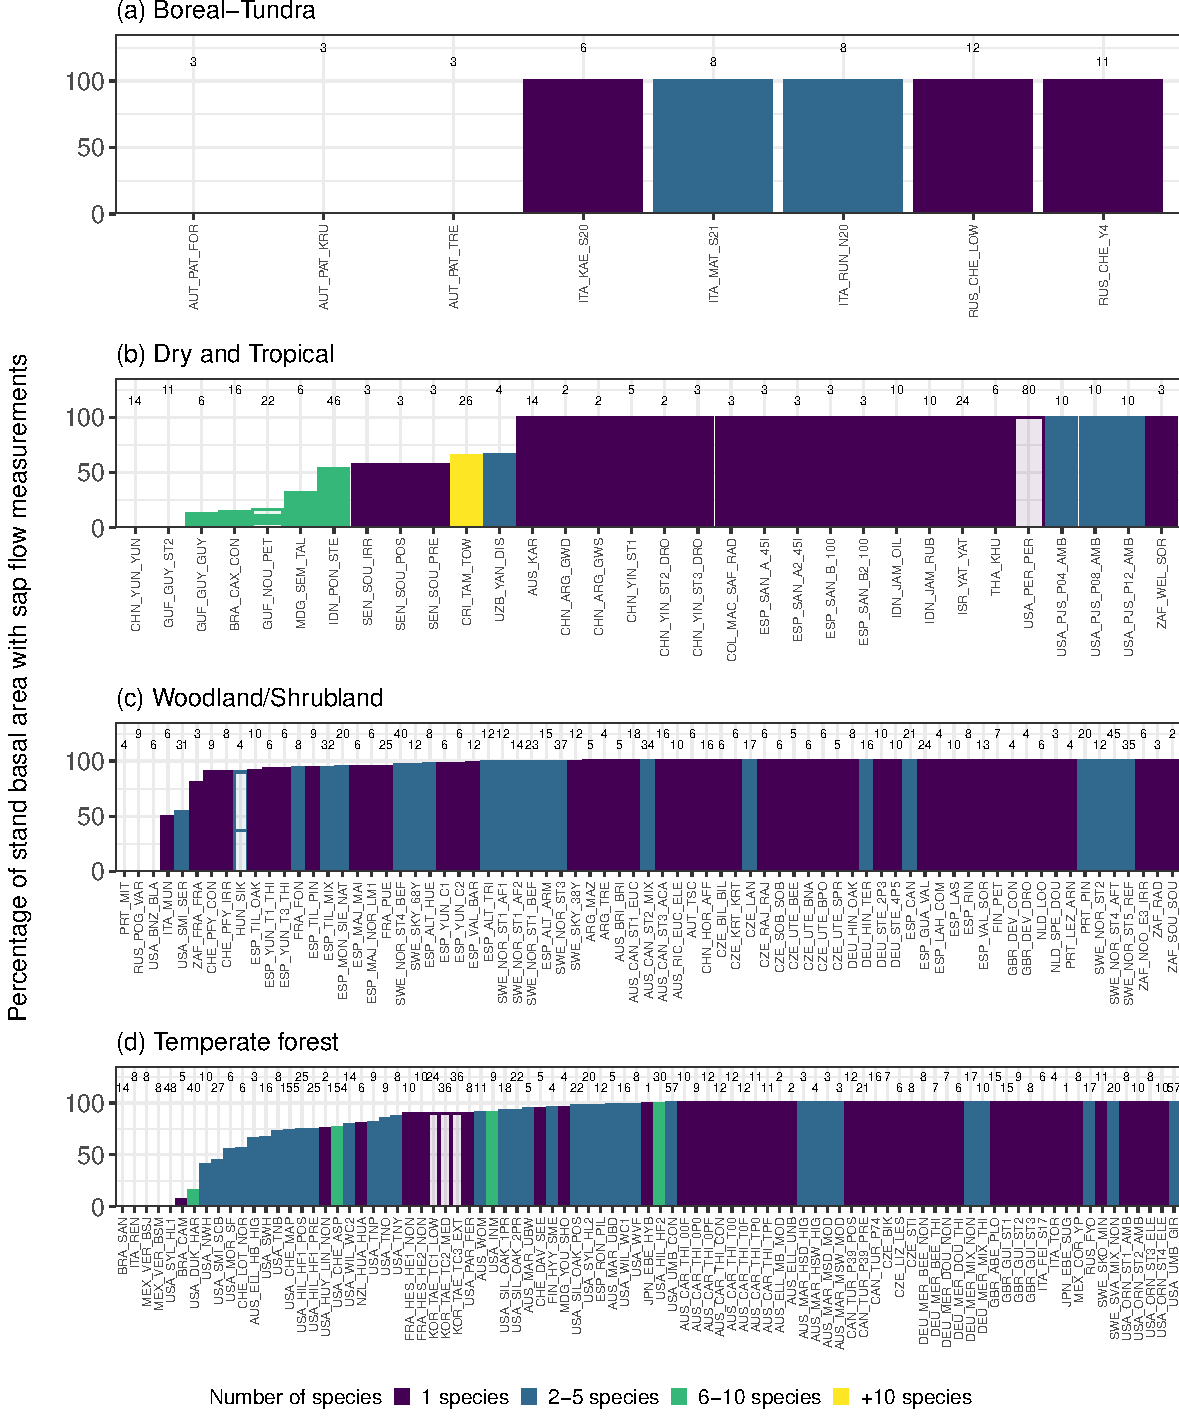
\includegraphics[width=1\linewidth]{figure/CH3/Figure9} 

}

\caption[Potential for upscaling species-specific plant sap flow to stand-level.]{Potential for upscaling species-specific plant sap flow to stand-level sap flow using SAPFLUXNET datasets. Datasets are shown using an aggregated biome classification; ‘Dry and Tropical’ include: ‘Subtropical desert’, ‘Temperate grassland desert’,‘Tropical forest savanna’ and ‘Tropical rain forest’. Each panel shows the percentage of total stand basal area that is covered by sap flow measurements for each species in the dataset. Datasets are also coloured by the number of species present. Numbers on top of each bar depict the total number of plants for a given dataset. Empty bars show datasets for which sap flow data expressed at the plant level were not available.}\label{fig:Ch2plot9}
\end{figure}
Stand-level transpiration estimates from a large number of SAPFLUXNET
sites can contribute to improve our understanding of the role of forest
transpiration in the context of stand water balance and its components
at the ecosystem (e.g.~Tor-ngern et al., 2018) and catchment levels
(Oishi et al., 2010; Wilson et al., 2001). Importantly, SAPFLUXNET can
contribute to better understand the global controls on vegetation water
use (Good et al., 2017), including the biological and climatic controls
on evapotranspiration partitioning into transpiration and evaporation
components (Schlesinger and Jasechko, 2014; Stoy et al., 2019). There is
some overlap between the FLUXNET network and SAPFLUXNET (47 datasets
from FLUXNET sites). Hence, transpiration from SAPFLUXNET can also be
used as a `ground-truth' reference for transpiration estimates from
remote sensing approaches (Talsma et al., 2018) and from eddy covariance
data (Nelson et al., accepted). Extrapolating sap flow-derived stand
transpiration to large spatial scales can be challenging due to
landscape-scale variation in forest structure (Ford et al., 2007) or
topography (Hassler et al., 2018), and to the low spatial
representativeness of sap flow measurements (Mackay et al., 2010). A
promising research avenue to help elucidate the role of vegetation in
driving hydrological changes across environmental gradients (Vose et
al., 2016) would be to combine species-specific stand transpiration data
from SAPFLUXNET with stand structural and compositional data from forest
inventories (e.g.~sapwood area index, Benyon et al., 2015).\par

Understanding the patterns and mechanisms underlying species
interactions with respect to water use within a community is necessary
to predict tree species vulnerability to drought (Grossiord, 2019).
Multispecies datasets from SAPFLUXNET (Table S4) can be used to assess
competition for water resources among species, for example by
identifying changes in seasonal water use across co-existing species and
hence characterizing the spatiotemporal segregation of their
hydrological niches (Silvertown et al., 2015). By providing a detailed
seasonal quantification of tree water use, SAPFLUXNET could also
complement isotope-based studies and contribute to interpret the large
diversity in root water uptake patterns observed worldwide (Barbeta and
Peñuelas, 2017; Evaristo and McDonnell, 2017) and to explain the
different seasonal origin of root-absorbed water across species and
environmental gradients (Allen et al., 2019).\par

Plant water fluxes and hydrodynamics are amongst the most uncertain
components of ecosystem and terrestrial biosphere models (Fatichi et
al., 2016; Fisher et al., 2018). These models are now incorporating
hydraulic traits and processes in their transpiration regulation
algorithms (Mencuccini et al., 2019), but multi-site assessments of
these algorithms are usually performed against evapotranspiration from
eddy flux data (Knauer et al., 2015; Matheny et al., 2014). Model
validation against sap flow data has been carried out typically in only
one (Kennedy et al., 2019; Williams et al., 2001) or few (Buckley et
al., 2012) sites. SAPFLUXNET can thus contribute to assess the
performance of models simulating transpiration of stands or species
within stands (e.g.~De Cáceres et al., submitted.), for a large number
of species and under diverse climatic conditions.\par

\section{Limitations and future
developments}\label{limitations-and-future-developments}

\subsection{Limitations}\label{limitations}

Sap flow data processing differs within and among methods, because
different algorithms, calibrations or parameters involved in sap flow
calculations may be applied. All of these methods contribute to
methodological uncertainty (Looker et al., 2016; Peters et al., 2018)
and this challenging methodological variability precludes the
implementation of a complete, standardised data workflow from raw to
processed data within SAPFLUXNET, as it is done for eddy flux data
(Vitale et al., 2020; Wutzler et al., 2018). Commercial software for sap
flow data processing from multiple methods is available
(i.e.~\url{http://www.sapflowtool.com/SapFlowToolSensors.html}) but it
has not yet been widely adopted. Freely available data-processing
software is only available for the HD method (Oishi et al., 2016;
Speckman et al., 2020; Ward et al., 2017).\par

Sap flow measured with thermometric methods provides a precise estimate
of the temporal dynamics of water flow through plants (Flo et al.,
2019). However, their performance in measuring absolute flows is mixed.
While some well-represented methods in SAPFLUXNET such as the CHP yield
accurate estimates (at least for moderate-to-high flows), the HD method,
the most represented method by far, can significantly underestimate
water flows (Flo et al., 2019). Because plant-level metadata contain
information that document the conversion from raw to processed data
(Appendix Table A5), a first-order correction for uncalibrated HD
measurements based on available methodological assessments can be
applied to allow intercomparability across methods. Nevertheless, given
the high unexplained variability (i.e.~by species and wood traits) in
the performance of sap flow calibrations (Flo et al., 2019), these
corrections should be applied with caution. The determination of zero
flow conditions (baselining) can also have significant impacts on the
quantification of absolute flow for several methods (Peters et al.,
2018; Smith and Allen, 1996; Steppe et al., 2010). The different
baselining approaches are also documented in the metadata to inform data
syntheses and/or to selectively apply correction factors.\par

SAPFLUXNET has been designed to store whole-plant sap flow data, and
therefore, sap flow measured at multiple points within an individual is
not available in the database. Even though this spatial variation could
be useful to describe detailed aspects of plant water transport
(Nadezhdina et al., 2009), focusing on plant-level data greatly
simplifies the data structure. Hence, SAPFLUXNET only includes data
already upscaled to the plant level by the data contributors. The main
details of how this upscaling process was done for each dataset are
provided together with other plant metadata (Table A5), but these
metadata show that within-plant variation in sap flow is often not
considered (Table 2). The impact of not accounting for radial and
circumferential variability when scaling single-point measurements of
sap flow to the whole-plant level can be important (Merlin et al.,
2020), but the estimation of sapwood area can also cause large errors
(Looker et al., 2016). SAPFLUXNET does not provide information on the
method employed to quantify sapwood area (e.g.~visual estimation with or
without the application of dyes, indirect estimation through allometries
at species or site levels) or on the accuracy of sapwood area data. This
precludes uncertainty estimation at the individual level. Future
developments in the SAPFLUXNET data structure could include this
information as metadata to better document the sensor-to-plant scaling
process.\par

While SAPFLUXNET makes global sap flow data available for the first
time, we note that spatial coverage is still sparse and some forested
regions are underrepresented in the database (Fig. 2a). We note
especially the relatively small number of datasets for boreal and
tropical forests, two important biomes in terms of global water and
carbon fluxes (Beer et al., 2010; Schlesinger and Jasechko, 2014). While
many geographic gaps are caused by the absence of sap flow studies from
such areas, some regions where sap flow studies have been conducted are
still not represented in SAPFLUXNET. For example, the recent
proliferation of Asian sap flow studies (Peters et al., 2018) has not
translated into a high representativity of Asian datasets in SAPFLUXNET
yet. Similarly, while the coverage of taxonomic and biometric diversity
is unprecedented, SAPFLUXNET lacks data for the extremely tall trees
(Ambrose et al., 2010) or for other growth forms such as shrubs (Liu et
al., 2011), lianas (Chen et al., 2015) and other non-woody species (Lu
et al., 2002).\par

\subsection{Outlook}\label{outlook}

The public release of SAPFLUXNET has set the stage for a first
generation of sap flow-based data syntheses. The work on these syntheses
will fuel new ideas and tools for future improvements of the database,
as for example new computing approaches for the processing and analysis
of sap flow datasets. One example would be the development of robust
imputation algorithms to gap-fill time series of sap flow and
environmental data, which can take advantage of tools and datasets
already developed by the ecosystem flux community (Moffat et al., 2007;
Vuichard and Papale, 2015). The dissemination of SAPFLUXNET will
encourage the use of machine-learning algorithms, only occasionally used
to analyse sap flow datasets so far (e.g.~Whitley et al., 2013). These
approaches can also be used to identify the relative importance of
different hydrometeorological drivers of transpiration (Zhao et al.,
2019), or to produce global transpiration maps, by combining SAPFLUXNET
with other data (Jung et al., 2019). This upscaling of stand
transpiration to large areas will also allow addressing broader
questions at the regional and continental scale, such as the role of
transpiration in moisture recycling (Staal et al., 2018).\par

The eventual success of this initiative, in terms of enabling data
reuse, contributing towards the understanding and modelling of tree
water use at local to global scales will likely encourage the sap flow
community to contribute new datasets to future updates of the database.
We expect that the development of open-source software for the
processing of sap flow raw data (Speckman et al., 2020), its eventual
widespread use by the sap flow community and the adoption of
standardized calibration practices will increase the quality and
intercomparability of future sap flow datasets. These new datasets will
hopefully expand the temporal, geographical and ecological
representativity of SAPFLUXNET when new data contribution periods can be
opened in the future.\par

\subsubsection{Change in niche size and species climatic
range}\label{change-in-niche-size-and-species-climatic-range}

The two first PCA axes explained 60.8\% of the variability of the 12
climatic variables (Appendix B Figure B.5). Lm models across species
with different distribution ranges showed that species with smaller
average-based niche area, which correspond to species with more
restricted distribution range, increased more their niche area when
considering inter-annual climatic suitability than species with larger
average-based niche area and wider distribution ranges (Figure 3.4 and
Appendix B Table B.3). In addition, there were no differences between
distribution range groups in the relationship of niche area ratio with
area of average-based species' niche (Appendix B Table B.3).\par

\section{Data availability, access and
feedback}\label{data-availability-access-and-feedback}

In this paper we present SAPFLUXNET version 0.1.5 (Poyatos et al.,
2020a), which contains some small metadata improvements on version
0.1.4, the first one to be made publicly available, in March 2020. Both
versions supersede version 0.1.3 which was initially released to data
contributors in March 2019. The entire database can be downloaded from
its hosting webpage in the Zenodo repository
(\url{https://doi.org/10.5281/zenodo.3971689}, Poyatos et al. 2020a). In
this repository, we provide the database as separate .csv files and as
.RData objects; see section 2.4. for details on data structure. Together
with the initial publication of SAPFLUXNET in March 2019, we also
released the sapfluxnetr R package, available on CRAN, to enable easy
access, selection, temporal aggregation and visualisation of SAPFLUXNET
data. Feedback on data quality issues can be forwarded to the SAPFLUXNET
initiative email address:
\href{mailto:sapfluxnet@creaf.uab.cat}{\nolinkurl{sapfluxnet@creaf.uab.cat}}.
All the information about SAPFLUXNET, including the publication of new
calls for data contribution, can be found in the project website:
\url{http://sapfluxnet.creaf.cat/./par}

\section{Conclusion}\label{conclusion}

The SAPFLUXNET database provides the first global perspective of water
use by individual plants at multiple timescales, with important
applications in multiple fields, ranging from plant ecophysiology to
Earth-system science. This database has been built from
community-contributed datasets and is complemented with a software
package to facilitate data access. Both the database and the software
have been implemented following open science practices, ensuring public
access and reproducibility. Data sharing has been a key component of the
success of the FLUXNET network of ecosystem fluxes (Bond‐Lamberty,
2018), and many databases in plant and ecosystem ecology now offer open
data (Bond-Lamberty and Thomson, 2010; Falster et al., 2015; Gallagher
et al., 2020; Kattge et al., 2020). SAPFLUXNET fully aligns with this
philosophy. We expect that this initial data infrastructure will promote
data sharing among the sap flow community in the future (Dai et al.,
2018) and will allow the continued growth of the SAPFLUXNET database.

\chapter*{References}\label{references}
\addcontentsline{toc}{chapter}{References}

Placeholder


% Index?

\end{document}
